%% $RCSfile: proj_report_outline.tex,v $
%% $Revision: 1.2 $
%% $Date: 2010/04/23 02:40:16 $
%% $Author: kevin $

\documentclass[11pt
              , a4paper
              , twoside
              , openright
              ]{report}


\usepackage{float} % lets you have non-floating floats

\usepackage{url} % for typesetting urls

%
%  We don't want figures to float so we define
%
\newfloat{fig}{thp}{lof}[chapter]
\floatname{fig}{Figure}

%% These are standard LaTeX definitions for the document
%%                            
\title{Interactive 3D Visualisation of Exoplanets}
\author{Owen Bannister, 300172912}

%% This file can be used for creating a wide range of reports
%%  across various Schools
%%
%% Set up some things, mostly for the front page, for your specific document
%
% Current options are:
% [ecs|msor]              Which school you are in.
%
% [bschonscomp|mcompsci]  Which degree you are doing
%                          You can also specify any other degree by name
%                          (see below)
% [font|image]            Use a font or an image for the VUW logo
%                          The font option will only work on ECS systems

\usepackage[font,ecs,mcompsci]{vuwproject}
\usepackage{graphicx}
\usepackage{pdfpages}
\usepackage{float}
  \usepackage{subfigure}
% You should specifiy your supervisor here with
     \supervisor{Dr Stuart Marshall}
% use \supervisors if there is more than one supervisor

% Unless you've used the bschonscomp or mcompsci
%  options above use
   \otherdegree{Bachelor of Engineering in Software Engineering with Honours}
% here to specify degree

% Comment this out if you want the date printed.
\date{}

\begin{document}

% Make the page numbering roman, until after the contents, etc.
\frontmatter

%%%%%%%%%%%%%%%%%%%%%%%%%%%%%%%%%%%%%%%%%%%%%%%%%%%%%%%

%%%%%%%%%%%%%%%%%%%%%%%%%%%%%%%%%%%%%%%%%%%%%%%%%%%%%%%

\begin{abstract}
Dr

Large amounts of information has been discovered about planets outside our solar
system, and this can be accessed by anyone from the Kepler
Exoplanets dataset \cite{datasetphl} \cite{dataset}. However this data is
complex and therefore not easily understood by laypeople who lack in depth
knowledge of stellar information. This is problematic as it
means that the data gathered about these planets is not being used
effectively to communicate to the masses. To resolve this a 3D interactive
visualisation called the Improved Kepler Visualisation Tool (IKVT) was created
by extending the exisiting Kepler Visualisation Tool to convey this information
in a way that
interested laypeople can understand. IKVT allows two methods of interaction by
keyboard \& mouse and by Microsoft Kinect sensor. This allows users, interested laypeople, to interact
with the visualisation via traditional means or by a more novel approach
respectively. This visualisation can be used as an
information source for those wanting to increase their knowledge about the
planets residing outside of our solar system. This report outlines the project
carried out and includes the planning of IKVT, its
implementation, and its user
evaluation to discover how effectively it fulfilled the system requirements
driving its
creation.


\end{abstract}

%%%%%%%%%%%%%%%%%%%%%%%%%%%%%%%%%%%%%%%%%%%%%%%%%%%%%%%

\maketitle

\chapter*{Acknowledgments}
I would like to thank Dr Stuart Marshall the supervisor of this project. He provided
me with endless advice and mentorship over the course of this project making it
a very positive experience. Thanks also goes to the Victoria University of
Wellington Human Computer Interaction Group who were always free to help and
provide me with assistance.


\tableofcontents

% we want a list of the figures we defined
\listof{fig}{Figures}

%%%%%%%%%%%%%%%%%%%%%%%%%%%%%%%%%%%%%%%%%%%%%%%%%%%%%%%

\mainmatter

%%%%%%%%%%%%%%%%%%%%%%%%%%%%%%%%%%%%%%%%%%%%%%%%%%%%%%%

% individual chapters included here
\chapter{Introduction}\label{C:intro}
This project seeks to design, implement, and evaluate an interactive 3D visualisation software system for displaying the content in the Kepler Exoplanets dataset. The deliverable is intended as a standalone 3D visualisation system with two modes of interaction, keyboard and mouse or Microsoft Xbox Kinect sensor ((REF)). The resulting visualisation will convey the information in the dataset in a way that the target users, laypeople who have an interest in astronomy, can understand and interact with.
\section{Motivation}
There are many planets that have been located outside of our own solar system, these are
called exoplanets, these are referred to interchangeably as planets and exoplanets for the remainder of this report
. This project seeks to develop and evaluate an interactive 3D visualisation
software system for the Kepler exoplanets dataset [28]. This visualisation will convey information
in a way that the target users, laypeople who have an interest in astronomy, can
understand.
\section{Problem statement}
The complex nature of the data involved in this project causes a range of problems revolving around understandability to arise, which this project attempts to address. The following subsections outline these in detail.
\subsection{Understanding the content in the dataset}
Understanding and analysing large datasets whose size defies simplistic or trivial analysis is a known issue that many areas of research are attempting to address, these areas of research range from data mining to visualisations in order to discover or highlight important features in the data so that people can more efficiently use it. 
\\\\
Humans often rely on visualisation when we solve problems. We create an image in our mind of a situation in order to make sense of it http://nrich.maths.org/6447.~ This allows for a much more comprehensive understanding of the content being visualised. The content in the dataset used for this project is made up of records of every exoplanet discovered by the Kepler Mission. Each of which contains 46 fields. It is next to impossible for someone to internally visualise so much information, most of which is floating point numbers.This means that an external way of visualising it is needed, which is the problem that this project attempts to address. 
\clearpage
\begin{figure}[h!]
  \centering
      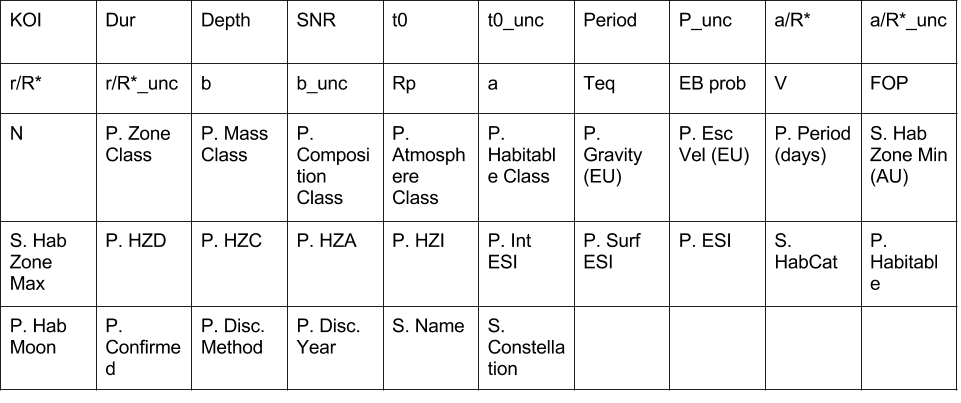
\includegraphics[width=0.8\textwidth]{images/data.png}
  \caption{Dataset to be visualised}
\end{figure}

\subsection{Comprehension of planetary information}
Much of the information regarding planets is cryptic and unintuitive, this make its understandability difficult. Visualisations in general attempt to address this issue by displaying information in a way that conveys the information in simplistic ways which allows improved user comprehension.

\subsection{Existing solutions lack functionality}
Existing data visualisation techniques using this exoplanet dataset lack the ability to display sufficient detail on each exoplanet and do not provide answers to questions that can be answered by the Exoplanet attributes in the dataset. Existing solutions display only the size, temperature, and orbital information about the exoplanets. While this is useful information that informs users of important facts about the planets, it does leave a lot of potential information unseen and overlooked, for example, information about the type of planet, planets with similar traits, solar system information, similarity to earth and habitability. This project will therefore be focused on researching, implementing, and evaluating a new interactive visualisation system that will display additional information to users not included in previous visualisation systems.

\subsection{Effective user interaction with visualisation}
A visualisation that solely displays information without effective methods of interaction limits the immersive qualities that keeps users engaged. To address this interactive visualisations emerged, generally these visualisations allow users to modify the representation of information rather than the information itself. This means allowing user control some property of how the data is represented, be it something simple as the layout of elements or something more complex. Many mediums of interaction are possible from the mundane keyboards, mice, or touchpads to the more esoteric wired gloves, motion sensors, and omnidirectional treadmills or even a combination of a range of devices.
\\\\
With interactive visualisations, response time of the system to user actions is important and so changes made by the user must be incorporated into the visualization in a timely manner. Experiments have shown that a delay of more than 20 ms between when input is provided and a visualisation is updated is noticeable by most people ((REFERENCE)~). Thus it is important for an interactive visualization to provide a rendering based on human input within this time frame or else risk breaking user immersion.
\\\\

When the information being presented is altered, the visualization is usually part of a feedback loop. For example, consider an aircraft avionics system where the pilot inputs roll, pitch, and yaw and the visualization system provides a rendering of the aircraft's new attitude. Another example would be a scientist who changes a simulation while it is running in response to a visualization (see Visualization) of its current progress. This is called computational steering.

\section{Key issues project addresses}
To summarize the above sections, this project addresses the following key issues:
\begin{enumerate}
 \item[I1.] Content in database form is difficult to view and understand.
 \item[I2.] Planetary information is complex and difficult to comprehend without a visual reference.
 \item[I3.] Existing visualisations for this dataset have minimal functionality and have lacking usability.
 \item[I4.] User interaction is needed in a visualisation to make the most of data displayed.
\end{enumerate}

\section{Contributions of this project}
This project will provide an extension of the Kepler Visualisation Tool \cite{kepler_github} that conveys more information and is easier for users to interact with than the original. This extension will be evaluated by a user experiment to ensure that it is successful in conveying the information contained in the dataset.
\\\\
The work and research completed for this project will allow for further improvement by other developers and researchers to extend and improve the visualisation created. This will provide further exposure of the Kepler dataset which will encourage learning about Exoplanets.


\chapter{Project Methodologies}\label{C:m}

\section{Project management approach}
Following a structured project management approach is important as it avoids the problem caused by following a code-and-fix approach as described  as 1) write some code. 2) Fix the problems in the code \cite{boehm}. By following a process model it encourages thinking about requirements, design, and testing before coding is commenced. 
\\\\
The project methodology chosen for this project was a customized Spiral Model made up of requirements analysis, design, implementation, and evaluation phases as shown in the below figure. The reason for limiting the model to these 4 phases was because....  
\begin{figure}[h!]
  \centering
      \includegraphics[width=0.6\textwidth]{images/spiral_model.png}
  \caption{Spiral process model followed}
\end{figure}
Using a spiral model allowed me to produce a deliverable feature at the end of each iteration of the model, this ensured that I did not become delayed or stuck in my development. By using this methodology it also allowed me to prioritize the features that were the most important to the visualisation which reduced the risk that there would be missing or incomplete components at the end of the project. 
\\\\
The advantages of this methodology over other choices such as the waterfall model or an agile approach such as Scrum was that it provided me with the benefits of a structured work flow that is a feature of the waterfall model as well as a flexible iterative process that is a feature of Agile methodologies. Following a pure waterfall methodology would not have allowed me to iteratively design, develop, and evaluate each feature which would have forced more upfront design which limits flexibility and support for changing requirements and design as was needed for this project. Following a pure agile approach would not have been optimal as most Agile methodologies are more beneficial to projects that have a team working on them. As it was I was agile in my approach to the project as I produced a deliverable at the end of each of the cycles of the spiral model and responded to change in the form of feedback and ideas from the supervisor of the project.
\\\\
This project management technique supported the creation of a visualisation as it allowed the flexibility to add and remove components into the visualisation as they were discovered to be beneficial or not. It also supported the expansion of the project brief to include using a kinect sensor in order to control the visualisation. The choice of this project management approach meant that whilst I had the freedom to explore visualisation options I also had a structured software development life cycle to guide me and provide the project through the necessary steps to end in completion of each component.
\\\\
By supporting this project methodology with other project management tools such as Gantt charts [APPENDIX] and work breakdown structures(WBS) [APPENDIX], it encouraged efficient documentation of planning and work completed in the project as well as displaying the upcoming stages required to complete the project.
\\\\
Weekly meetings with the supervisor of the project, Dr Stuart Marshall, were used to provide guidance and ideas for innovation of the visualisation throughout the project. These meeting ensured that vital components and deliverables were implemented in the required timeframe and also provided a sounding board for ideas for elements to be included in the visualization. Another important aspect of having an involved supervisor was that he provided me the guidance of an experienced academic which was indispensable when navigating the administrative side of organizing delicate matters such as ethics approval for human evaluation of the visualisation.


\section{Key difficulties in project}
As this project builds upon a previous system much of the existing code and execution flow needs to be modified. This requires understanding of how the system was originally built and designed. Because this system does not have any unit or integration tests, going ahead without a comprehensive knowledge of the core functionality would be foolish.
\\\\
Encountered errors in Processing framework due to number of elements needing to be displayed on screen. 
\\\\
Having a time constraint of 300 hours for this project over the course of a year meant that prioritization of visualization features needed to be made to ensure that 
\\\\
Libraries used for gesture detection in kinect are opensource in order to work with processing did not have decent detection
\chapter{Requirements Analysis}\label{Chap:ra}
To guide the creation of the visualisation a user oriented design approach was
used \cite{AboutFace3}, in particular making use of user models (personas). These personas were
created to give a sense of empathy and understanding for the foreseen users of
the visualisation in order to better understand the requirements and design
decisions to be made. 

The visual design of the visualisation was based heavily on User Centered Design as it
provided a method of user interface design as well as visualisation design. User
Centered Design is a process in which the needs, wants, and limitations of the
end users of a system are given extensive attention. To achieve this, personas
were created (also known as archetypal users), which are a personification the
needs of a larger group of related users. These personas act as stand-ins for
real users, describing them in terms of their goals and personal
characteristics, and although they are fictitious, they are based on knowledge
of real users. This design methodology supported my understanding of how users
were likely to use the visualisation.

An additional tool used during requirements analysis was User Scenarios which
describe the foreseeable interactions of the user personas with the
visualisation. A scenario is made up of a functional goal for the visualisation
and describes how it is carried out by a persona. Both of these tools force you
to think about the tasks needed for the visualisation and their context in the
system as a whole. Once the personas and scenarios have been completed you can
then start to design specific elements of the user interface and visualisation
based on the requirements and interactions described in the scenarios. The User
Models and User Scenarios for this project are described in the following
sections.


\section{User models}
Below are the two personas that were used in the design of the visualisation for
this project. They depict users that would use the visualisation in the context
of a terminal or display in an observatory environment. These personas  can be
validated during evaluation of the visualization by finding real users that
match the core values of the personas.Although this visualisation would be
suited towards teaching childeren about stelar information they were not
focussed on during its planning. This was because due to the increased ethical
complexity with carrying out an evaluation with childeren. This could be done in
the future once the visualisation is deemed successfull. 

\subsection{John Truman (Primary Persona - The interested layperson)}\
24 year old John is interested in planets and space and has a basic knowledge
about both. He frequently visits attractions catering to this interest at
locations such as planetariums and observatories. Some of his favourite things
to do when visiting these attractions is to go to the computer terminals that
allow users to choose what information they see.

John is used to playing computer games and using visualisations and is not
overwhelmed understanding and using new systems. He finds that he learns better
when provided with visual examples than when reading or listening to
information. John is most comfortable using keyboard and mouse when interacting
with a computer.

\subsubsection{Scenario 1: View planets ordered by their similarity to Earth}
 When John first sees the system the first thing he notices is that there are
many planets orbiting what looks like a star. He doesn't have any point of
reference for these planets so their sizes, colours, and movement speeds are
meaningless. By providing a way of comparing the planets to Earth it gives a
point of reference which is well documented and known by most.
 
 {\bf Procedure:}
 \begin{enumerate}
 \item John selects that he wants to view the exoplanets compared by their
similarity to earth.
 \item The planets on screen move so that they are placed in a way that John can
compare them to Earth.
 \item From here John can select any of the planets for further analysis.
 \end{enumerate}

  \subsubsection{Scenario 2: Select ranges for attributes of each planet
displayed}
 John has become comfortable with selecting the planets and has some idea of the
scale and basic attributes of the planets. Now he wants to select more planets
to find out more information. However due to the large number of planets he
finds it difficult to accurately select them due to overlapping and fast moving
small planets.
 
  {\bf Procedure:}
  \begin{enumerate}
 \item John uses a range of filters to remove planets from his view that don't
match the criteria he chooses (temp ,size ,KOI , ESI).
\item As planets disappear the graph of planets expands into the space that
frees up, this causes more space to appear between planets making them more
selectable.
 \end{enumerate}
 
  \subsubsection{Scenario 3: Select planets to display more information}
 John wants to see more information about each of the planets he can see
orbiting in the visualisation. To do this he wants to be able to select the
planets and have textual information appear on screen.
 
  {\bf  Procedure:}
   \begin{enumerate}
 \item John has the option to pause the rotation of planets in order to make
more accurate selections. 
 \item John clicks on a planet orbiting a planet.
\item The planet selected becomes larger and its outline grows, making it more
visible.
\item The text window has all of the information about the planet selected added
to it.
 \end{enumerate}
 
 \subsubsection{Scenario 4: View planets in the same solar system}
John is curious about which of the planets he can see in the
visualisation are in the same Solar System. To discover this he wants that when
a planet is selected all other planets in the same Solar System as the selected
planet to become highlighted.
 
  {\bf  Procedure:}
   \begin{enumerate}
 \item When John selects a planet, all planets in the same Solar System become
more visible.
 \item A label appears on these planets indicating that they are related
planets.
 \end{enumerate}
 
  
 \subsubsection{Scenario 5: View the Goldilocks zones of each exoplanets star}
   Looking at the planets orbiting the sun in the visualisation John wonders
whether any of them could support life. To see this John wants to see which
planets are in the habitable zones of their stars. 
 
  {\bf  Procedure:}
   \begin{enumerate}
 \item John selects that he wants to view the exoplanets compared to their stars
habitable zones.
 \item The habitble zones of the selected planets star become visible.
 \item When a planet from a different star system is clicked then the habitable
zones will change to match the new selected planets stars habitable zones.
 \end{enumerate}
 
  \subsubsection{Scenario 6: Select two planets to compare against one another}
When John is selecting planets to view more information he often finds that he
wants to compare his selections against another planet. To do this John wants to
be able to make multiple selections to compare two planets against one another.
  
  {\bf  Procedure:}
   \begin{enumerate}
 \item John selects a planet and chooses to compare it against another planet.
 \item Information about this second planet appears so that John can make
comparisons.
  \end{enumerate}

\subsection{Cara Thompson (Secondary Persona - Likes gesture based systems)}
23 year old Cara likes using interactive visualisations when visiting
attractions, she finds that they are more entertaining and provide a better
level of interaction and more of a novelty experience with a visualisation than
simply a keyboard and mouse. 
\\\\
Both of these users are similar in their need for information from the
visualisation but differ in the methods that they wish to access the information
and interact with the visualisation. John wants to interact with keyboard and
mouse as it is more straight forward and accurate. Cara wants to interact with
gestures as she finds it more of a novelty and more immersive.

 \subsubsection{Scenario 3: Select planets to display more information}
 Cara wants to see more information about each of the planets she can see
orbiting in the visualisation. To do this she wants to be able to hover her hand
over a planet to get the information to display on screen.
 
  {\bf  Procedure:}
   \begin{enumerate}
 \item Cara hovers her hand over a planet to make a selection
 \item The planet selected becomes larger and its outline grows, making it more
visible.
\item The text window has all of the information about the planet selected added
to it.
 \end{enumerate}
 
 \subsubsection{Scenario 4: View planets in the same solar system}
Cara is curious about which of the planets she can see in the
visualisation are in the same Solar System. To discover this she wants that when
a planet is selected all other planets in the same Solar System as the selected
planet to become highlighted.
 
  {\bf  Procedure:}
   \begin{enumerate}
 \item When John selects a planet, all planets in the same Solar System become
more visible.
 \item A label appears on these planets indicating that they are related
planets.
 \end{enumerate}

 \subsubsection{Scenario 7: Navigate the visualisation with gestures}
Cara doesn't find using keyboard and mouse interesting enough for interacting
with the visualisation. She would rather navigate around the visualisation by
using hand
gestures as it's more immersive.

  {\bf  Procedure:}
   \begin{enumerate}
 \item By moving her hand the visualisation pans
in the corresponding direction, ie if the hand goes to the top of the screen
the visualisation pans up.
 \item By moving her hand backwards and forwards the visualisation will zoom in
and out.
  \end{enumerate}
  
  
\section{Requirements summary}
\subsection{Functional Requirements}
Functional requirements define the functions of a system and are derived from
the scenarios described above. These functions are
described as a set of inputs, the behavior, and outputs from the system. The
functional requirements for this visualisation are as follows:
\begin{enumerate}

 \item[R1.] The visualisation needs to display planetary information to convey
knowledge to
users.

 \item[R2.] The visualisation needs to allow exoplanets to be compared against
one another.

 \item[R3.] The planets need to be able to be ordered by their similarity to
earth (ESI) and by their Kepler Object of Interest number (KOI).
 
 \item[R4.] The visualisation needs to allow users to define ranges of planetary
attributes to filter which planets are displayed.

 \item[R5.] Users need to be able to view the habitable zones of stars in
relation to the planets orbiting them.

\end{enumerate}

\subsection{Nonfunctional Requirements}
 Functional requirements are supported by non functional requirements. Non
functional requirements impose constraints on the design or implementation (such
as performance, security, or usability) of a system.
 
 The non functional requirements for this visualisation are as follows:
\begin{enumerate}
 \item[R6.] All interaction methods must be visible and intuitive.

 \item[R7.] The visualisation must remain uncluttered to reduce information
overload.

 \item[R8.]  There needs to be two modes of interaction with the system,
keyboard and mouse vs gesture based.
\end{enumerate}

%matrix
\begin{figure}[H]
  \centering
      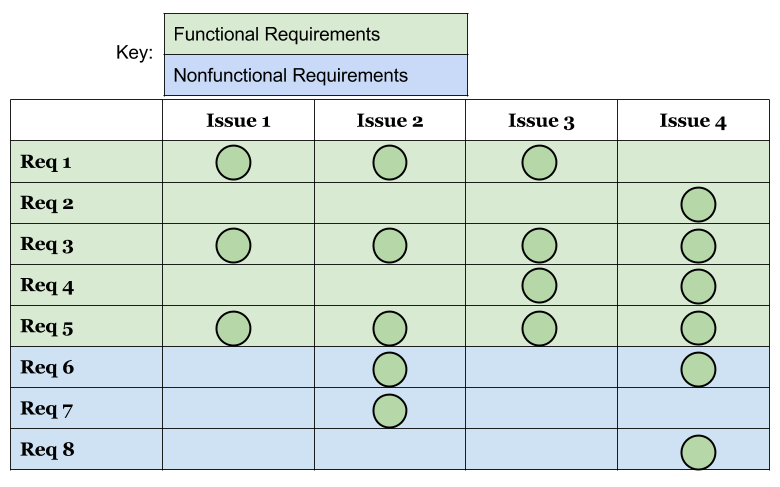
\includegraphics[width=1\textwidth]{images/issues_to_req_matrix.png}
  \caption{Matrix of project requirements to issues project is attempting to
address}
\end{figure}

\chapter{Related Work} 
This section discusses 4 existing visualisations that have a theme revolving
around
space or planets. Following a short description, each visualisation is analysed
to
discover which of the User Scenarios detailed in the previous chapter exist
within the
system.

\section{Worlds: The Kepler Planet Candidates - Non Interactive}
Worlds \cite{worlds} displays planet candidates found by NASA's Kepler
mission. These candidates are animated in orbit around a single star. They are
drawn to scale with accurate radii, orbital periods, and orbital distances. They
range in size from 1/3 to 84 times the radius of Earth. Colors represent an
estimate of temperature with red indicating warmest, and blue indicating coldest
candidates. 
\begin{figure}[H]
  \centering
      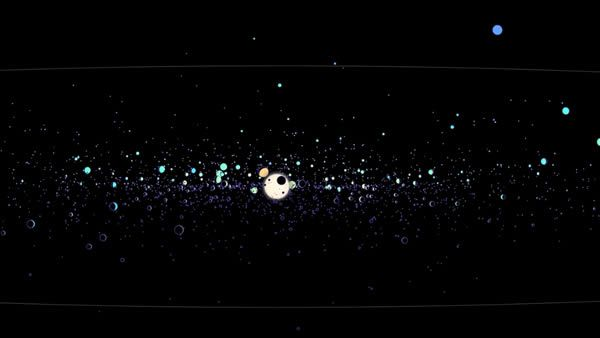
\includegraphics[width=0.8\textwidth]{images/worlds.jpg}
  \caption{Image of Worlds Visualisation}
\end{figure}
Worlds has a visually appealing layout that effectively displays the basic
attributes of each planet. By examining this visualisation we can see how
displaying the planets orbiting a single star allows users to visually make a
basic comparison between each planet. The below paragraphs discuss the User
Scenarios that Worlds fulfills.
 \\\\
{\bf Scenario 1. View planets ordered by their similarity to Earth:\\}
Worlds has comprehensive functionality for comparing the different exoplanets to
one another, however it does not offer any functionality regarding comparisons
to earth 
\\\\
{\bf Scenario 2. Select ranges for attributes of each planet displayed:\\}
Worlds doesn't offer any functionality for any filtering of exoplanets, this
means that users can only see all planets at once which can be overwhelming and
causes exoplanets to be excluded from view due to overlapping
and clustering. The reason that this is done is to convey how many exoplanets
there are and how their scale differs among on another.
\\\\
{\bf Scenario 3. Select planets to display more information:\\}
Worlds is non interactive meaning that users are not able to request further
information about the visualisation elements that they are seeing. This ability
to find out more is a key part of the interactive visualization needed
for this project.

\section{The Kepler Orrery and The Kepler Orrery 2 - Non interactive}
The Kepler Orrery \cite{orrery} illustrates exoplanets in their
own solar systems. The orbit radii are to scale with respect to each other and
planet sizes are to scale with respect to each other, but orbits and planet
sizes are different scales. The colors are in order of semi-major axis:
two-planet systems (242 in all) have a yellow outer planet; 3-planet (85) green,
4-planet (25) light blue, 5-planet (8) dark blue, 6-planet (1, Kepler-11)
purple. 
\begin{figure}[H]
  \centering
      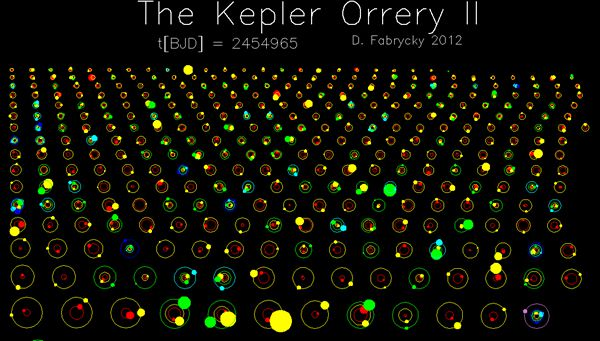
\includegraphics[width=0.8\textwidth]{images/orrery.jpg}
  \caption{Image of The Kepler Orrery Visualisation}
\end{figure}
This system exhibits small multiples, a grid of small similar graphics or
charts, allowing them to be easily compared. This provides insights into how I
can use small multiples to display information about groups of planets. This
will be important for displaying which planets share a solar system. The below
paragraphs discuss the User Scenarios that The Kepler Orrery fulfills.
\\\\
{\bf Scenario 1. View planets ordered by their similarity to Earth:\\}
Like Worlds, The Kepler Orrery shows the similarities between each of the
exoplanets but does not have the functionality to allow users to make a
comparison to earth and our own solar system.
\\\\
{\bf Scenario 4. View planets in the same solar system:\\}
The layout of the visualisation uses small multiples to group each solar system
of exoplanets and stars together which removes the issue of overcrowding and
overlapping elements. Displaying each exoplanet
orbiting its own star removes the risk of confusion about what planets are
actually orbiting which could be the case with Worlds.

\section{Celestia - Interactive}
Celestia \cite{celestia} is a 3D space simulation written in C++. Celestia does
not include any stars that are more than a
few thousand light-years from the Sun because the distant
stars are too small difficult to measure, meaning that it doesn't contain
the distant exoplanets discovered by the Kepler mission. 
\begin{figure}[H]
  \centering
      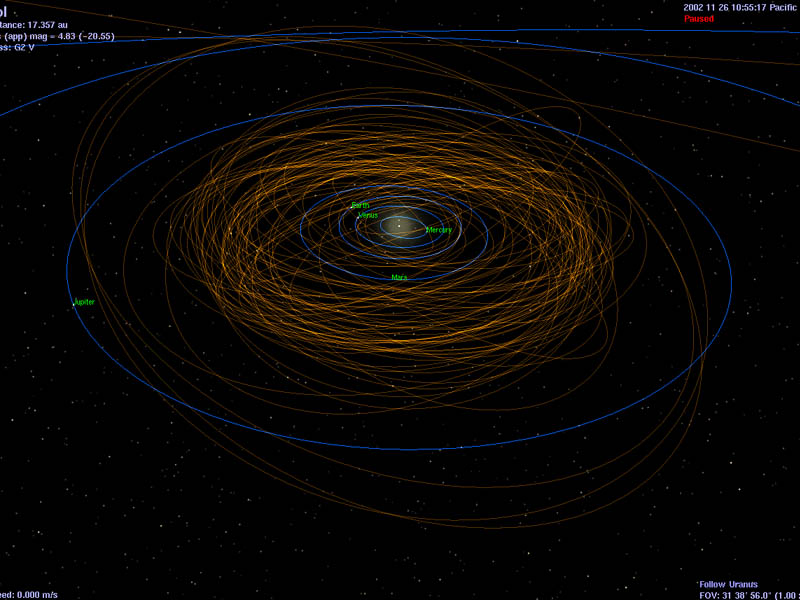
\includegraphics[width=0.8\textwidth]{images/celestia.jpg}
  \caption{Image of Celestia Visualisation}
\end{figure}
This visualisation is much larger and more encompassing system than is needed
for this project, as it is a full simulation. However is does offer
insights into how to effectively portray planets and their orbits (See Figure
2.3). It also provides textures that can be used to depict
what planets look like to increase user immersion. The below paragraphs discuss
the User Scenarios that Celestia fulfills.

{\bf Scenario 3. Select planets to display more information:\\}
Celestia allows users to view a large set of information about each of the
planets that it displays. The information is available in toolbars
that can be accessed. Examples of this information are radius, phase angle,
rotation speed, and temperature of planets.  
\\\\
{\bf Scenario 4. View planets in the same solar system:\\}
Celestia allows users to explore a range of solar systems their planets. This is
a key feature of the experience that
Celestia tries to give users, ie letting them explore the vastness of space in a
3D simulation. 

\section{Kepler Visualisation Tool}
\label{sec:kep}
The Kepler Visualisation tool \cite{kepler_github, kepler_article} is a 3D
visualisation built with Processing (A Java library and development
environment). It is a simple visualisation focusing
on displaying the estimated size, orbital speed, and orbital
separation of each exoplanet. All exoplanets are color-coded to visually
represent
their estimated temperatures.
\begin{figure}[H]
  \centering
      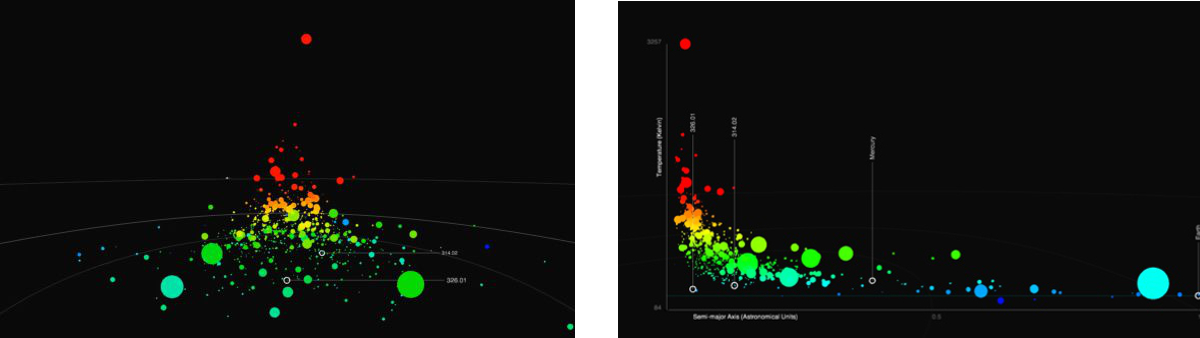
\includegraphics[width=1\textwidth]{images/kepler.jpg}
  \caption{Kepler Visualisation Tool Orbital View}
\end{figure}

The existing work in this system would serve as foundation for this project as
much of the visual aspects, and initial data manipulation of this visualisation
is already complete. It means that implementing the features
needed for this project could be focused on more heavily, and larger
improvements could be undertaken. The below paragraphs
discuss the User Scenarios that Kepler Visualisation Tool fulfills.
\\\\
{\bf Scenario 1. View planets ordered by their similarity to Earth:\\}
Like Worlds and the Kepler Orrery, The Kepler Visualisation Tool has
functionality to display the similarity of each Exoplanet to each other.
However, it also has some limited functionality of comparing these to earth
which the others lack. It does this by displaying Earth, Mars, and Jupiter by
the same method as the Exoplanets. This gives users a point of common reference
with which to make comparisons.
\\\\
{\bf Scenario 2. Select ranges for attributes of each planet displayed:\\}
The Kepler Visualisation Tool allows users to sort the exoplanets on the Y axis
by their size and temperature, but does not allow users to specifiy ranges of
these to filter them.
\section{Summary of Existing Applications}
\begin{figure}[H]
  \centering
      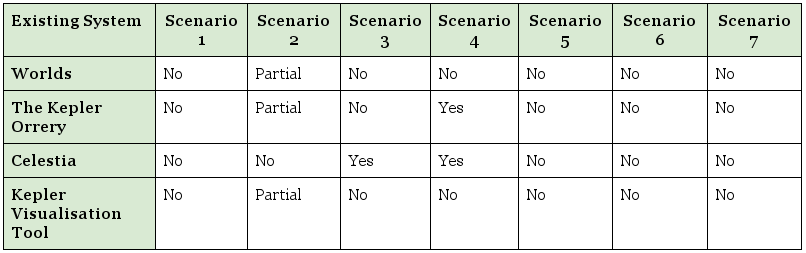
\includegraphics[width=1\textwidth]{images/existing.png}
  \caption{Matrix of existing solutions mapped to scenarios}  
    \label{fig:existing}
\end{figure}



\chapter{Technology} 

Many technologies were examined and experimented with as the candidates for the basis of the visualisation tool. Then the positives and
negatives of each was weighed up before a decision about the
suitable choice was made. It came down to three potential
technologies, the next three subsections outline these in
detail.

\section{Processing - Chosen Technology}
Processing \cite{processing} is an open source programming language and development environment
that was created to teach the fundamentals of computer programming with a visual
context.
Using processing would mean that the visualization could be built with Java
while still using
an effective visualisation framework that supports 3D elements. The most
complete existing visualization
using
the same exoplanet dataset (The Kepler Visualization Tool) is built using
Processing.
Using this solution would involve learning the semantics of Processing but as it
is a library built in Java so the syntax is only slightly different.
This means the learning
curve should be shallow.

\section{D3 (Data Driven Documents) - Alternate Technology}
D3 \cite{d3} is a JavaScript library that allows the data to be displayed in dynamic
graphics. Embedded
within an HTML web page, the JavaScript D3.js library uses pre-built
functions to
select elements, create Scalable Vector Graphics (SVG)objects, style them,
and add transitions,
dynamic effects, and tooltips. Large datasets can be easily bound to SVG objects
using
simple D3 functions to generate rich charts and diagrams. D3 was created because
of the
need for a balance of expressiveness, efficiency, and accessibility that
previous visualisation
toolkits did not allow [4].

D3 allows the binding of input data to arbitrary input elements. This means that
the exoplanet dataset can easily be bound to SVG elements to create a
visualisation. D3
adopts the W3C Selectors API to identify document elements queried. This results
in a
rich but concise selection method of elements in a visualisation. It allows
debugging due to Google Chrome and other modern browser
development tools. A downside to D3 is that it does not allow 3D diagrams,
although it does
allow pseudo 3D by using the painters algorithm and 3D textures.

\section{Prefuse - Alternate Technology}
Prefuse is a set of software tools for creating rich interactive data
visualizations \cite{prefuse}. The
Prefuse toolkit provides a visualisation framework for Java. It supports a set
of features
for visualising and interacting with data. It can be used to build standalone
applications, visual
components embedded
in larger applications, and web applets. Prefuse greatly simplifies the
process
of representing and efficiently handling data, mapping data to visual
representations (e.g.
through spatial position, size, shape, color, etc), and interacting with the
data.
To use Prefuse a basic familiarity with the Java is required, including setting
up and building
Java projects. A knowledge of Swing or another similar user interface toolkit is
also
useful for understanding some of the concepts behind Prefuse and for integrating
Prefuse
visualisations into larger applications. Prefuse is a very powerful tool that
has a very high learning curve due
to the amount of development power that it has. This means that learning it and
using it pushed it out of scope for this project.


\section{Decision of Technology}

The technology chosen needed to offer a combination of low learning curve,
strong visualisation ability, and 3D support.
The final decision was to use Processing, this is because it had all
of the desirable qualities that this project required as Figure \ref{fig:
techChoices} shows. 

\begin{figure}[H]
  \centering
      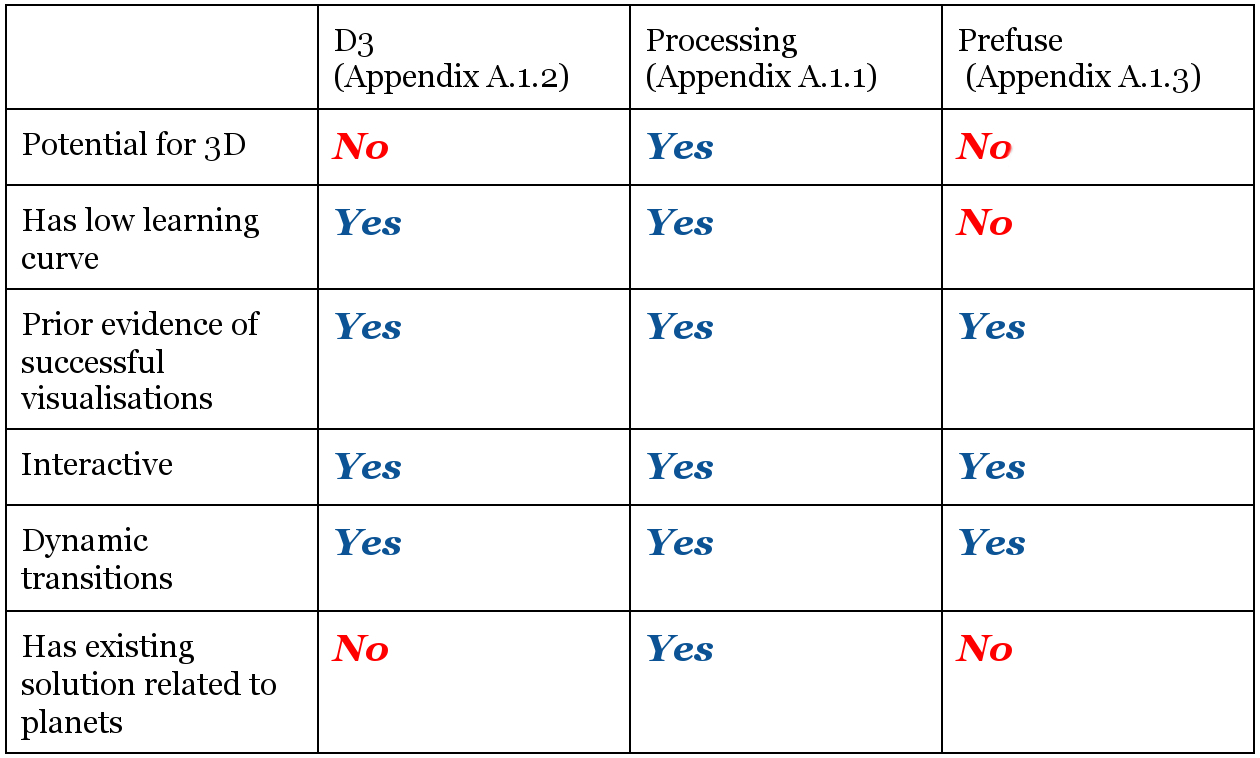
\includegraphics[width=0.8\textwidth]{images/table_technologies.pdf}
  \caption[Matrix of technology options to desirable qualities]{Matrix of technology options to desirable qualities that solve the issues this project addresses. We can see that Processing is the most suitable as it satisfies each of the desirable qualities followed by D3 and then Prefuse}
  \label{fig: techChoices}
\end{figure}

Choosing Processing as the development tool allowed me to extend an existing visualisation
using the same data set, The Kepler Visualisation Tool in Section \ref{sec:kep}.
Building upon an existing solution allowed the project to progress faster
towards fulfilling the project requirements as less of the groundwork needed to
be carried out. This was a large advantage as doing this groundwork would limit
the amount of time spent on new features.



\chapter{Solution Design: Improved Kepler Visualisation Tool (IKVT)}\label{C:sd}
This section discusses the design of the deliverable visualisation, The Improved
Kepler Visualisation Tool(IKVT). It details
the key design decisions revolving around structure, aesthetics, and
functionality that were made about the visualisation. 
% Description of tool
This project aims to improve an existing visualisation, The Kepler Visualisation
Tool which was discussed in the previous chapter. Whist this existing
visualisation displays exoplanets and some of their features, it lacks
interactivity for users trying to use it to gain information contained in the
Kepler Exoplanet Database effectively. The IKVT expands on this pre-existing
visualisation by adding key elements of interactivity missing in the existing
 visualisation as well as further enhancing the range and amount of data that
is available to users about exoplanets. The IKVT also incorporates a novel
gesture based interactive mechanism to the visualisation.

\section{System design and structure}
Because this project builds upon an existing system complete comprehension of
how it is designed and how it functions is important. Going ahead in the
creation of the visualisation without this knowledge would create opportunities
for mistakes and incorrect assumptions about how the visualisation needs to be
created. To assist with this issue the following two tools were used.

\begin{enumerate}


 \item UML Sequence Diagram
  \\image\\description of\\what it shows about visualisation
   \begin{figure}[H]
  \centering
      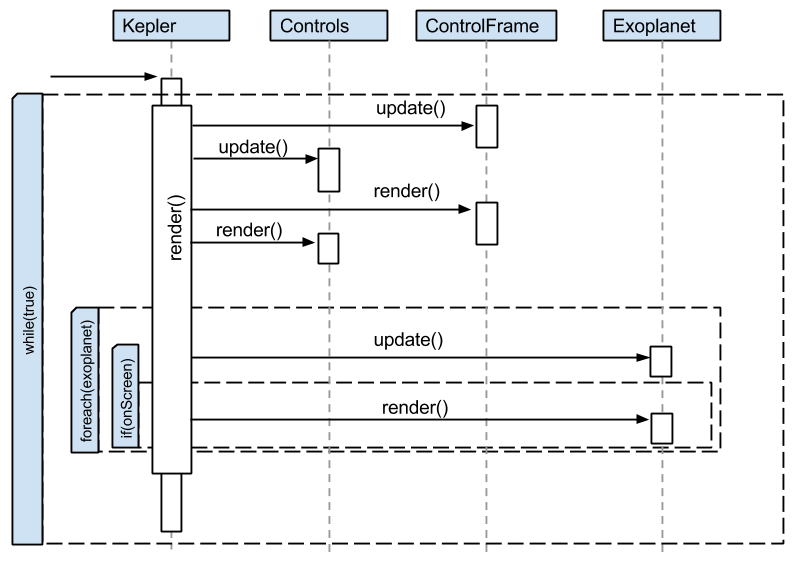
\includegraphics[width=0.8\textwidth]{images/sequence.png}
  \caption{Sequence Diagram of IKVT render cycle}  
\end{figure}

 \item UML Class Diagram
 \\image\\description of\\what it shows about visualisation
 \begin{figure}[H]
  \centering
      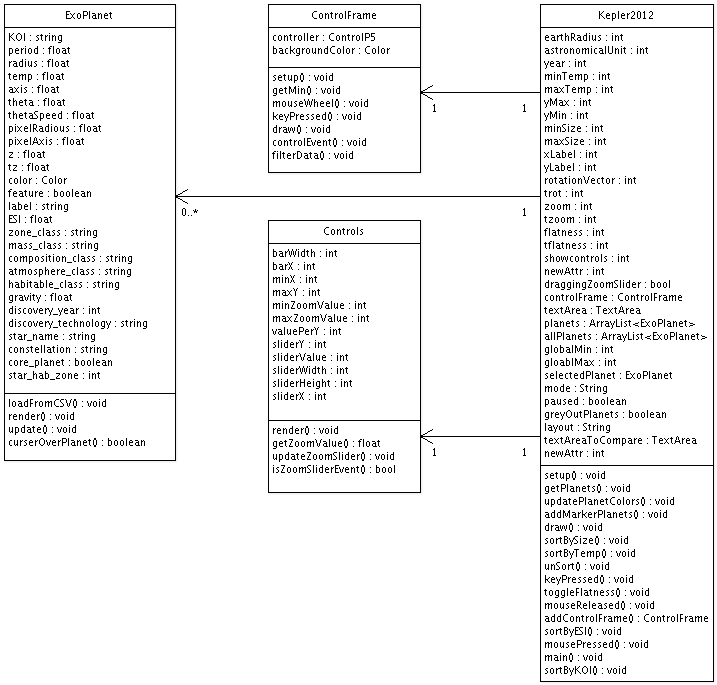
\includegraphics[width=0.8\textwidth]{images/classDiagram.png}
  \caption{Class Diagram of IKVT}  
\end{figure}
 

\end{enumerate}

\section{Visualisation Design}
The requirements produced in the Requirements Analysis chapter provide a
description of the functionality that needs to be designed for this
visualisation. By adding additional details to these requirements we can design
how the visualisation should look, behave, and function.

By using abstract user interface design the layout and configuration of each
element can be
planned and coordinated without the need for excessive details which are likely
to change
throughout the course of the project (e.g. colours and content) \cite{martin}.

\subsection{Functional Requirement}
\begin{enumerate}
{\bf
 \item[R1.] The visualisation needs to display planetary information to convey
knowledge to users.
}

  This requirement needs some form of textual display in order to convey enough
of the information about exoplanets to the user. The most obvious choice for
this would be to use a Java TextArea object to display each of the key
attributes of each Exoplanet. The following figure is a mockup of the text area
showing the information about each planet that will be displayed and the method
calls that will be used.

\begin{figure}[H]
  \centering
      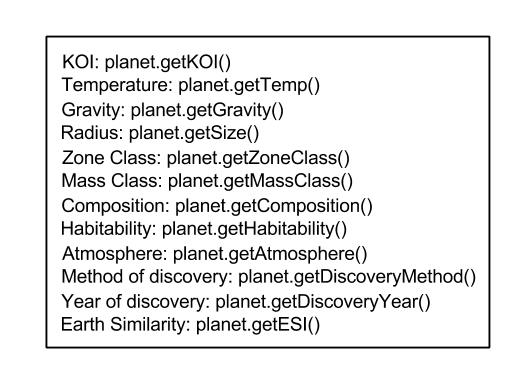
\includegraphics[width=0.8\textwidth]{images/textAreaMockup.png}
  \caption{Mockup of the text area}  
\end{figure}

SELECTIONG ~
All planets need to be selectable and react appropriately when
clicked.

To fulfill this requirement every planet needs to be able to be selected. This
involves detecting when a user clicks and then finding whether any planets are
located in that space. This is more complex in this system as it requires
detecting where each planet is in a 3D space and checking whether the 2D
location of the mouse click coincide. 

When a planet is successfully selected it needs to provide feedback and
information to the user to inform them that it has been selected and also to
provide relevant information.

\begin{figure}[H]
  \centering
      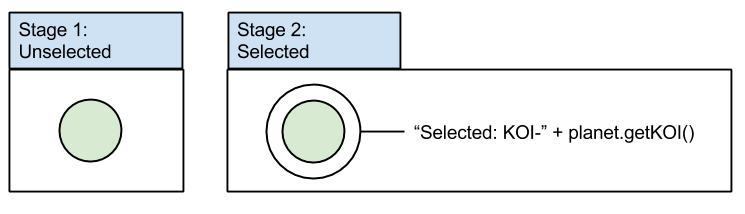
\includegraphics[width=.8\textwidth]{images/mockSelected.png}
  \caption{Mockup selection process}  
\end{figure}

When a planet is selected all other planets in the same solar system
need to become more visible.

When a planet has been successfully selected all of the other planets in the
same solar system (sister planets) need to become highlighted. This can be done
by treating them as if they were selected and providing an additional indication
that they are not actually selected.  
\begin{figure}[H]
  \centering
      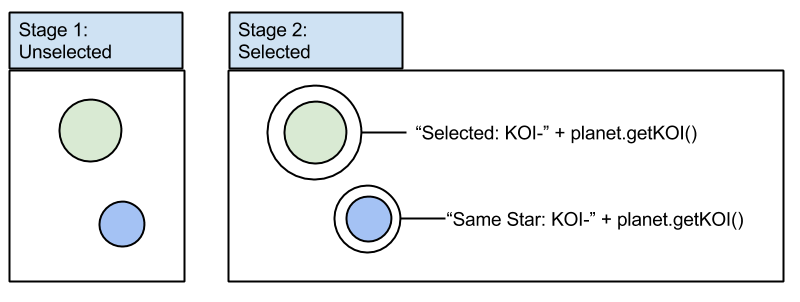
\includegraphics[width=.8\textwidth]{images/selectedSisterPlanets.png}
  \caption{Mockup highlight sister planets process}  
\end{figure}

{\bf
 \item[R2.] The visualisation needs to allow exoplanets to be compared against
one another.}

\begin{figure}[H]
  \centering
      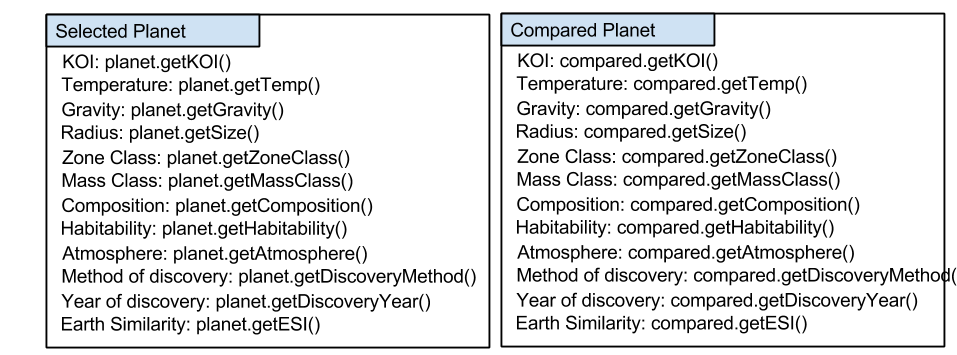
\includegraphics[width=.7\textwidth]{images/mockComparePlanets.png}
  \caption{Mockup compare planets text areas}  
\end{figure}

Using each of the previously discussed elements of interacting with the
visualisation this requirement is fulfilled. The text areas coupled with the
main visualisation window mean that all of the important and valuable
information about each exoplanet can be conveyed to a user.

{\bf
 \item[R3.] The planets need to be able to be ordered by their similarity to
earth (ESI) and by their Kepler Object of Interest number (KOI).}

To fulfill this requirement the visualisation needs to allow users to view the
exoplanets in a way that uses the Earth as a point of reference and their Earth
Similarity Index (ESI) to order them and control their position. The following
figures display an abstract mockup of how this would be done.

\begin{figure}[H]
  \centering
      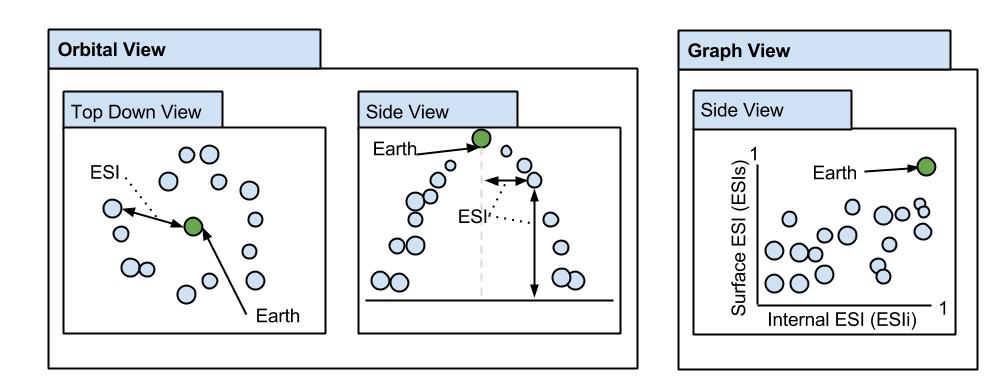
\includegraphics[width=1\textwidth]{images/mockupESI.png}
  \caption{Mockup of ESI views}  
\end{figure}


{\bf
 \item[R4.] The visualisation needs to allow users to define ranges of planetary
attributes to filter which planets are displayed.}

To fulfill this requirement a method of filtering exoplanets by their attributes
in order to control the number and types of planets displayed to the user. A
common method of achieving this is to use a set of sliders that allow a user to
filter something by a set of values. For example in this system a slider could
be used to control the size of planets that are displayed.

\begin{figure}[H]
  \centering
      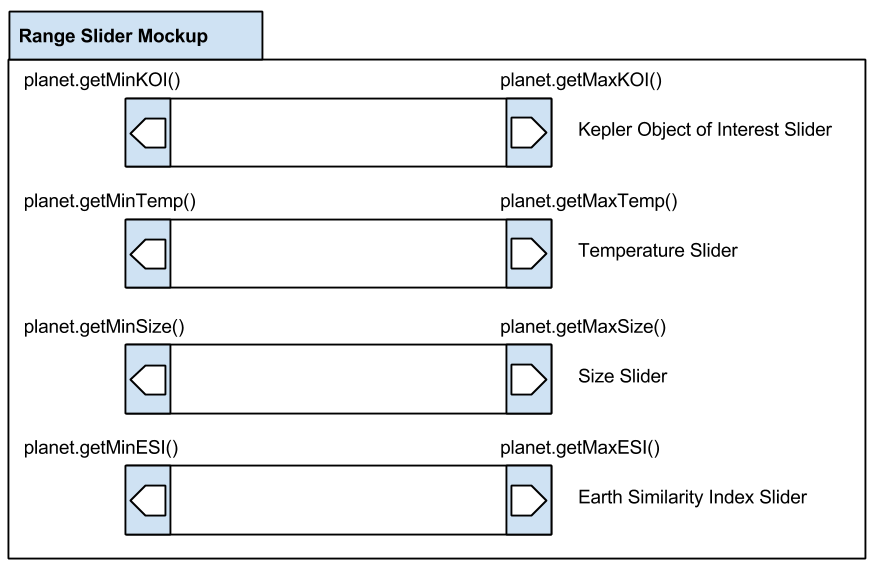
\includegraphics[width=.8\textwidth]{images/mockSlider.png}
  \caption{Mockup of range sliders}  
\end{figure}



{\bf
 \item[R5.] Users need to be able to view the habitable zones of stars in relation to the planets orbiting them.}

\begin{figure}[H]
  \centering
      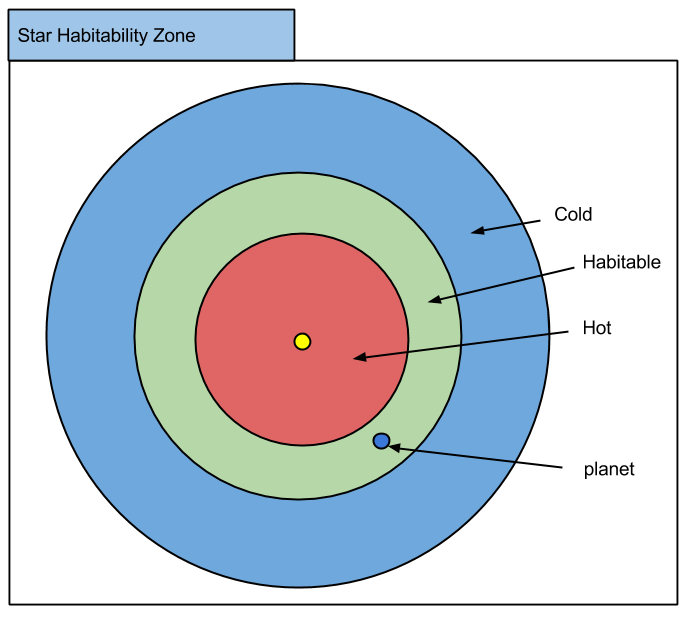
\includegraphics[width=.5\textwidth]{images/mockStarHabitability.png}
  \caption{Mockup star habitability zone}  
\end{figure}




\end{enumerate}

\subsection{Nonfunctional Requirement}

\begin{enumerate}


{\bf \item[R6.] All interaction methods must be visible and intuitive.}
\begin{figure}[H]
  \centering
      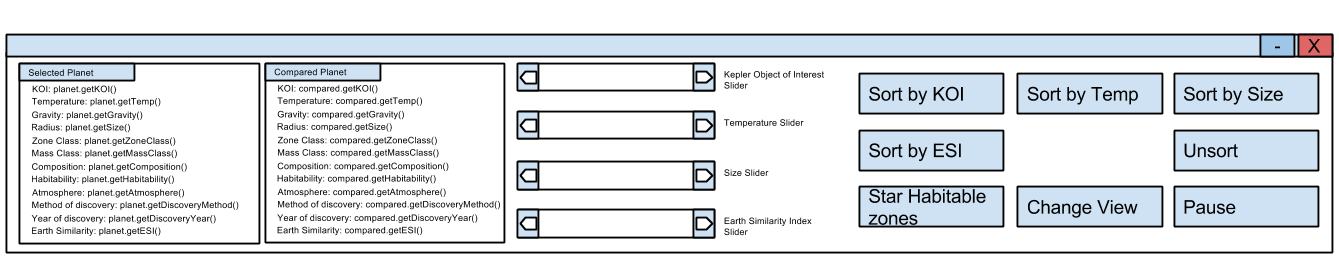
\includegraphics[width=1\textwidth]{images/allTogether.png}
  \caption{Mockup of the interaction panel}  
\end{figure}

 The visualisation needs to have a range of interactive buttons for
each element of interactivity in the system to help inform users how to use the
system.

\begin{figure}[H]
  \centering
      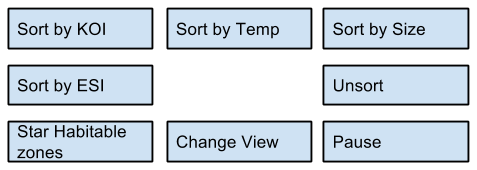
\includegraphics[width=0.5\textwidth]{images/mockButtons.png}
  \caption{Mockup of interactive buttons}  
\end{figure}

{\bf \item[R7.] The visualisation must remain uncluttered.}

By separating each of the interactive components into a separate window inside
the visualisation it provides 

The visualisation must not show so much information that it
causes information overload for users.

The ability to filter and sort the exoplanets gives a user the tools needed to
reduce the quantity of planets displayed in the visualisation and thus the
information load imposed on users. 
In addition to this, by having the text area that displays the information about
selected planets separate from the main visualisation it reduces the cognitive
load on users as they don't have to use this component until they want to. ~


{\bf  \item[R8.] There needs to be two modes of interaction with the system,
keyboard and mouse vs gesture based.}

The above requirements mostly relate to the keyboard an mouse system although some of the requirements do carry through to the Microsoft Kinect system as well. 

For the Kinect system the key difference is that the user will be able to control the main visualisation window with gestures. This means incorporating a means of detecting the gestures. 
\begin{figure}[H]
  \centering
      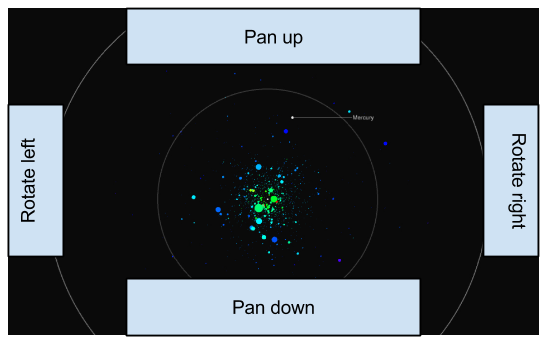
\includegraphics[width=0.7\textwidth]{images/mockKinect.png}
  \caption{Mockup of the Kinect system}  
\end{figure}

As the Kinect sensor no longer requires the use of a mouse the visualisation
design needs to be modified to accommodate the use of gestures. This meant incorporating new cursors to indicate the state of the visualisation.
There are 7 states that the cursor needs to be able to be in to inform the user
of what action they are performing. These states are

\begin{enumerate}
 \item default cursor, hand is at rest
 \item panning up, hand is raised
 \item panning down, hand is lowered
 \item rotating left, hand is to the left
 \item rotating right, hand is to the right
 \item zooming in, hand is pressed forward
 \item zooming out, hand is pulled backwards
\end{enumerate}
\begin{figure}[H]
  \centering
      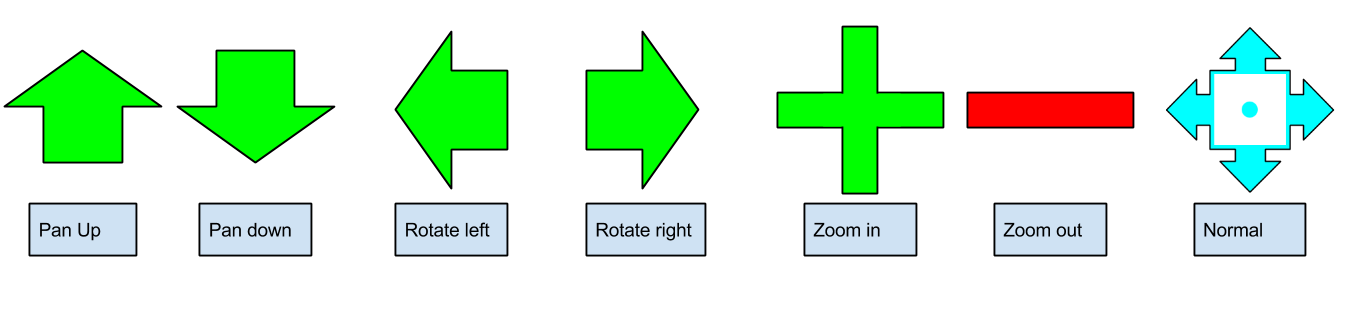
\includegraphics[width=0.9\textwidth]{images/curserImages.png}
  \caption{Mockup of cursor images for Kinect system}  
\end{figure}

Having a range of icons that clearly display these states is vital for keeping
the user informed of what they are doing. The icons designed for this purpose
are in the following figure

\begin{figure}[H]
  \centering
  ~
      %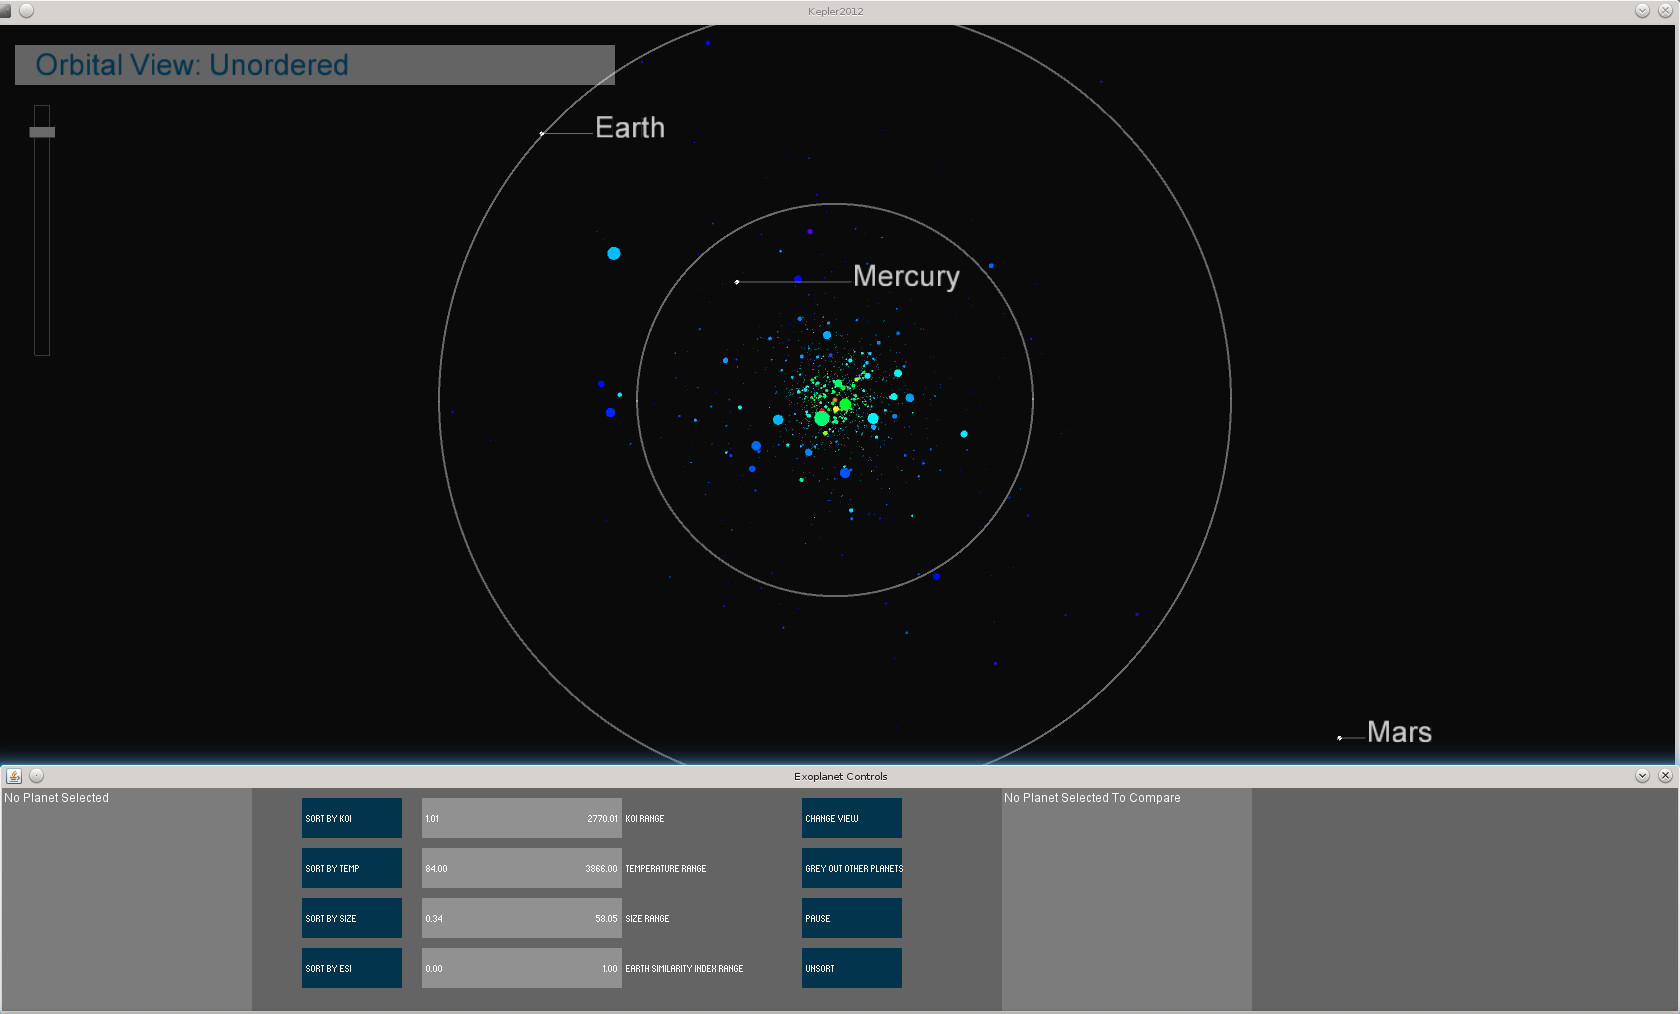
\includegraphics[width=0.8\textwidth]{images/layout_horizontal.jpg}
  \caption{Cursors for Kinect sensor}  
\end{figure}


\end{enumerate}



\chapter{Visualisation implementation of the Improved Kepler Visualisation Tool
(IKVT)}\label{C:imp}
This chapter discusses the implementation of the visulisation using the designs
from Chapter \ref{C:sd} to fulfill the requirements of this project.
It details the tools used, the deliverable features
produced, and the problems encountered. 

\section{Tools and Artifacts Used}
\subsection{Keyboard \& Mouse System}
In addition to Processing there was an additional open-source
library required for effective user interface components called ControlP5
\cite{controlp5}. This library provides customisable and intuitive user
interface components. It allows for the creation of visually appealing and
precisely
aligned interactive GUI components.

\subsection{Microsoft Kinect System}
For the Microsoft Kinect version of IKVT two additional libraries were required
to integrate the Kinect sensor
with Processing, these were:
\begin{enumerate}
 \item NITE \cite{nite}.
 \item SimpleOpenNi \cite{simpleopenni}.
\end{enumerate}
These libraries provided drivers to run the Kinect sensor in Processing
(SimpleOpenNi) as well
as basic gesture recognition and body tracking (NITE). However these libraries
were
opensource options due to the official Microsoft Kinect SDK not being compatible
with
Processing. This meant the gesture recognition was not as user friendly or
effective as the
official libraries. The effect of this was that the gesture tracking used in the
system had to be created sup-optimally from the open-source libraries which took
more time and resources. 

\section{Implementation of IKVT}

IKVT displays all 2234 exoplanets
in the Kepler exoplanets dataset \cite{dataset}. Each of these exoplanets are
represented as coloured
ellipses, of which the colour and size are representative of the exoplanets
temperature and size respectively. IKVT displays all of these exoplanets as if
they are orbiting a single star. In reality this would result in planetary
collisions, but in this visualisation provides users with a way to effectively
make observations and comparisons about each of the exoplanets in a single
view. 

There are two panels that make up the visualisation: the visualisation panel,
and the control panel. The visualisation panel is where the exoplanets
are displayed along with a text box describing the state of the visualisation
to
keep the user informed. The control panel contains all of the interactive
components that the user can use to change the state of the visualisation. The
components it contains are; two text areas that can be used interchangeably to
display information about selected planets (Requirement 1), four range sliders
(Requirement 4) shown in Figure 
\ref{fig:sliders} that are used to
filter the exoplanets as discussed previously, and eight buttons to toggle the
state of the visualisations. These buttons are ``Sort by KOI'', ``Sort by Temp'',
``Sort by Size'', ``Sort by ESI'', ``Change View'', ``Suns Habitable Zone'', ``Pause'',
and ``Unsort'' as shown in Figure: \ref{fig:buttons}. 

\begin{figure}[H]
  \centering
      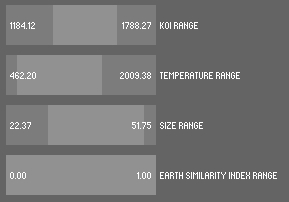
\includegraphics[width=0.6\textwidth]{images/sliders.jpg}
  \caption[Implementation of interactive range sliders]{Implementation of
interactive range sliders a various stages of filtering. The light grey bar in
the center of the sliders is the range of the attributes selected to filter by.
These can be modified by clicking and dragging on either end of the filter to
change the ranges, or selecting the middle to move the selected range up and
down the continuum}
  \label{fig:sliders}
\end{figure}

\clearpage
\begin{figure}[H]
  \centering
      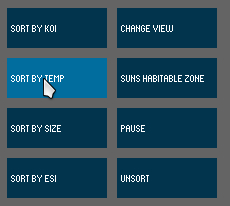
\includegraphics[width=0.6\textwidth]{images/buttons.jpg}
  \caption[Implementation of interactive buttons]{Implementation of interactive
buttons, each one of which corresponds to a key functionality in the
visualisation}
  \label{fig:buttons}
\end{figure}

Detailed information can be accessed about each exoplanet by clicking on them in
the main visualisation window to
make a selection. To do this a user can click on any of the orbiting exoplanets.
The effect of this selection is that a text box will have further textual
information about the selected exoplanet appended to it. In addition to this
users have the option of clicking a button labeled ``Compare''. This allows
the user the option to select another exoplanet so that its information is
appended to a second text area (Requirement 2). This can be seen in Figure
\ref{fig:textBoxes}. 
\clearpage
\begin{figure}[H]
  \centering
      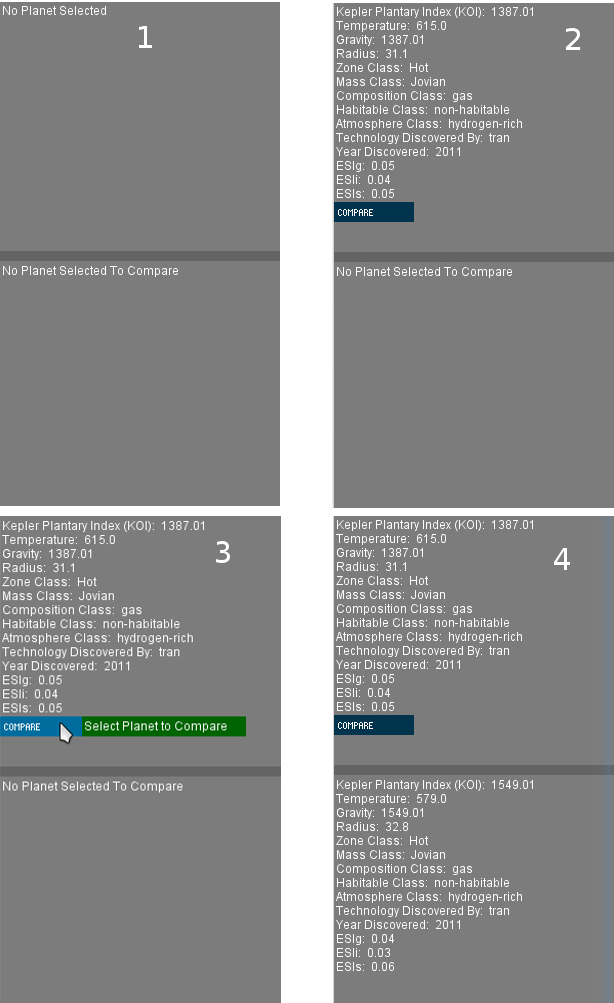
\includegraphics[width=0.7\textwidth]{images/textBoxes.jpg}
  \caption[Implemented text areas in each possible state]{Implemented text areas
in each possible state, Stage 1: No selection has been made so boxes are empty,
Stage 2: A single exoplanet has been selected and its information is displayed
as well as the option to compare, Stage 3: The user has chosen to compare the
selected exoplanet to another, Stage 4: A second exoplanet has been selected and
its information added to the second text area.}
  \label{fig:textBoxes}
\end{figure}
When a user is unable to accurately select an
exoplanet due to the clustering or
overlapping of exoplanets they can move the camera around in space to gain a
better viewing position. If this is not
enough, the user can use a set of range selectors to filter the exoplanets
displayed, as shown in Figure \ref{fig:zoomFilter}. The exoplanets can be
filtered by their KOI,
temperature, size, and ESI. These filters allow for
users to fine tune the exoplanets they wish to view, thus allowing them to work
with small multiples rather than the entire dataset. Using
these filters also causes a zooming effect to occur as exoplanets are filtered
out.
This zooming occurs each time the filters are changed as the exoplanets spread
out vertically and allows more space between them to make selections.

\begin{figure}[H]
  \centering
      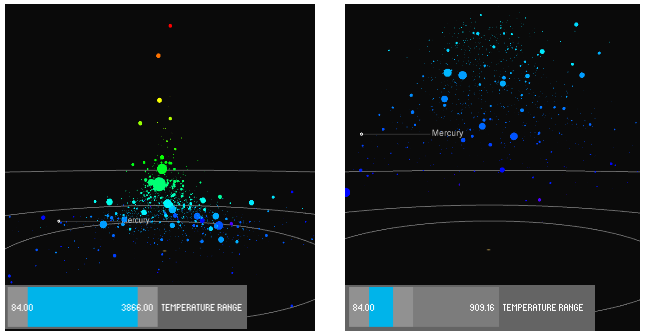
\includegraphics[width=0.8\textwidth]{images/zoomFilter.png}
  \caption[Zooming effect provided by filtering]{The above images display the
zooming effect provided by filtering. In the left image we can see that the
filters have not been used yet and all exoplanets are present which causes
clustering. In the right image the range has been  shrunk to filter out hot
exoplanets. This causes the colder planets to take up the space that was
originally occupied by all exoplanets which allows them to spread out.}  
    \label{fig:zoomFilter}
\end{figure}

The existing Kepler Visualisation Tool allowed users to sort the exoplanets on
the Y axis by their temperature and size. In IKVT this has been extended to
allow sorting by KOI and ESI (Requirement 3)as shown in Figure \ref{fig:ESIKOI}.


\begin{figure}[H]
  \centering
      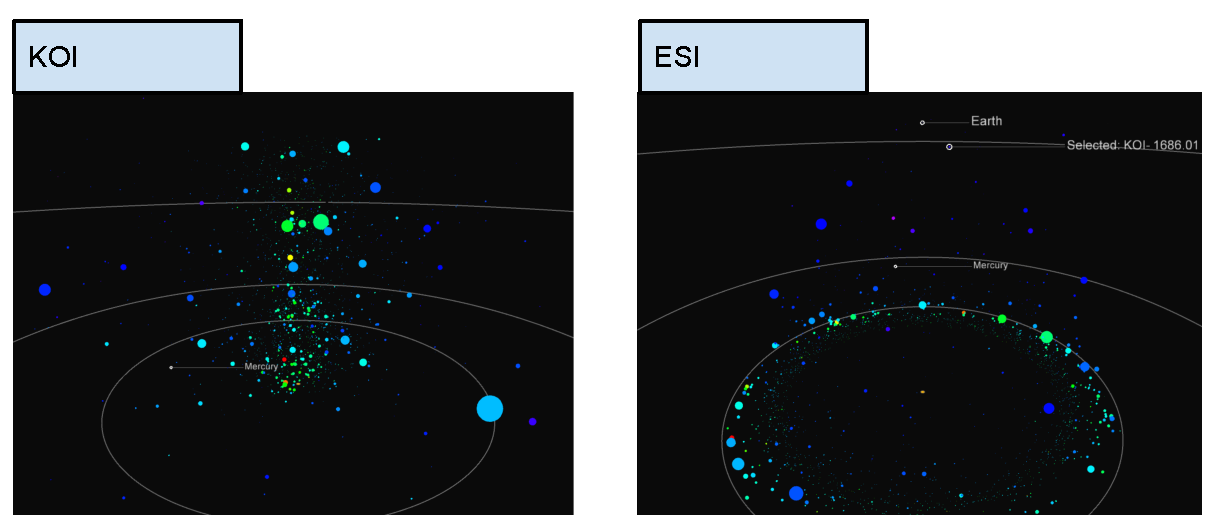
\includegraphics[width=1\textwidth]{images/ESIKOI.pdf}
  \caption[Implementation of sort by KOI and ESI]{The above images display the
implementation of sort by KOI and ESI. The left image shows the exoplanets sorted on the Y axis
by their KOI, this allows users to get an idea of which exoplanets share a solar
system as they will have similar KOI values. In the right image exoplanets are
sorted by their ESI on both the Y and X axis so that planets closer to the
center and the top are most similar to Earth}  
    \label{fig:ESIKOI}
\end{figure}

When a exoplanet is selected it is important that the user gets feedback about
what they have done. In IKVT this happens in the form of the selected exoplanet
becoming larger and a white outlining ring expanding out to encircle it. In
addition to this a label appears to the right of the exoplanet stating the
KOI. 

\begin{figure}[H]
  \centering
      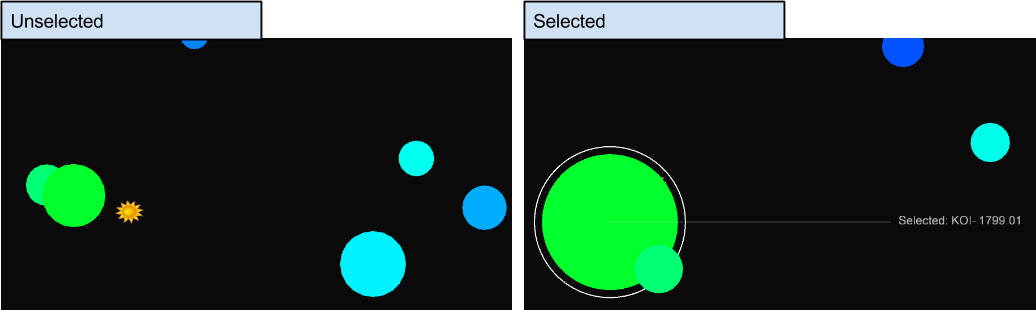
\includegraphics[width=1\textwidth]{images/selectedPlanet.jpg}
  \caption[Implementation of the exoplanet selection process]{The above images
display the implementation of the exoplanet selection process. We can see the
result of an exoplanet being selected, first the planet expands, then a white
circle expands out to outline it and a label appears to inform the user about
the exoplanet they selected.}  
    \label{fig:selectedPlanet}
\end{figure}

Another effect of a user making a selection is that all exoplanets that share
the same star as the selected exoplanet also become highlighted in the
same way as outlined above. The only difference is that in the label to the
right
of each exoplanet the message now informs the user that it has the ``Same
Star'' as displayed in Figure \ref{fig:sameStar}.

\begin{figure}[H]
  \centering
      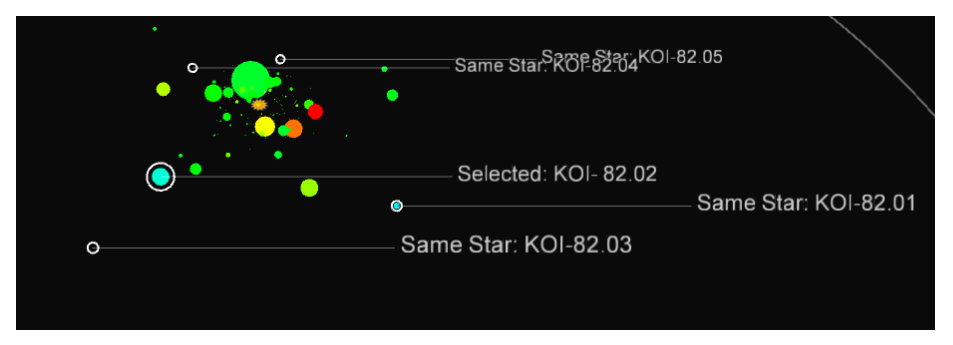
\includegraphics[width=1\textwidth]{images/sameStar.png}
  \caption[Implementation of exoplanets in the same solar system]{This image
displays how the planets in the same solar system as a selected planet become
highlighted in the same way but with a different label.}  
    \label{fig:sameStar}
\end{figure}


To display the Goldilocks zone of selected exoplanets coloured rings appear to
display the habitable
and inhabitable zones of the star (Requirement 5). Each time a new planet is
selected the
coloured rings change to represent the newly selected exoplanet's star, this can
be seen in Figure
\ref{fig:habitable}. In addition to the coloured rings the selected planet also
becomes highlighted
and all of the other exoplanets become transparent making it stand out to help users understand
whether it is in a habitable zone or not.

\begin{figure}[H]
  \centering
      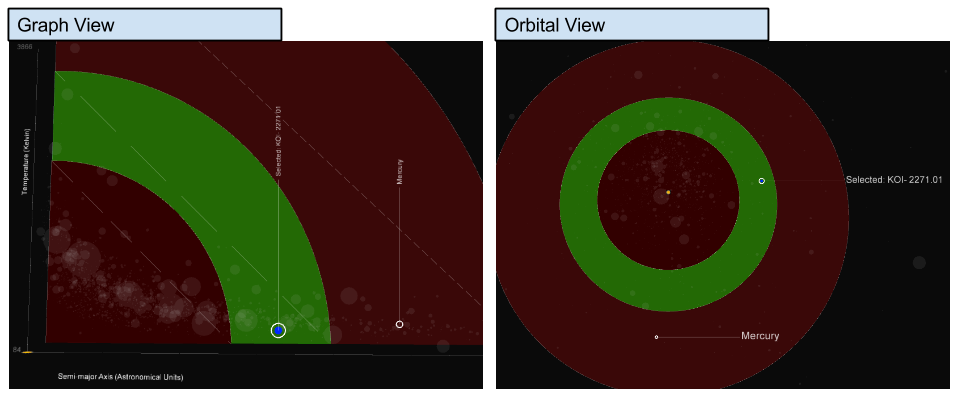
\includegraphics[width=1\textwidth]{images/habitable.png}
  \caption[Implementation of Goldilocks zones]{This image displays the
implementation the view Goldilocks zones feature which show how the coloured
rings are used, and how the planets relation to them infers their habitability.}
  
    \label{fig:habitable}
\end{figure}

Each of these implemented elements need to be visually apparent and intuitive to
use to ensure that the system can be
easily used without prior experience. This is done by providing clearly
labeled interactive elements and tooltips explaining what they
do as in Figure \ref{fig:tooltip}. These tooltips are widely used as a method of
informing a
user about the purpose of an item by hovering over it removing the need to
click on a button to discover its effect.

\begin{figure}[H]
  \centering
      
\includegraphics[width=0.8\textwidth]{images/tooltip.jpg}
  \caption[Tooltip on hover]{This image displays the implemented tooltips which
allow users to hover over interactive elements to discover what they do which
removes the need to
click on a button to discover its effect}
  \label{fig:tooltip}
\end{figure}

Due to the need for effective user interaction with the visualisation, a window
is required to house all of the components discussed above. Having this window
spatially separated from the main visualisation window means that users will not
be drawn away from the visualisation by overlapping and intrusive controls. Each
of the controls discussed above are included in this panel as shown below in
Figure \ref{fig:nav}.
\clearpage
\begin{figure}[H]
  \centering
      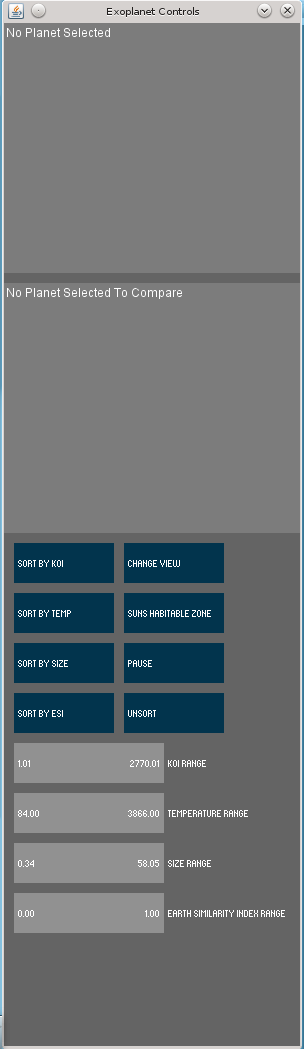
\includegraphics[width=0.3\textwidth]{images/nav.png}
  \caption[Implementation of Control Panel]{Shows the implemented Control Panel
that contains all of the interactive components discussed previously.}
  \label{fig:nav}
\end{figure}

At first the visualisation was laid out so that the control panel took up a
300 pixel strip along the bottom of the screen with the main visualisation
window
taking up the rest of the space as in Figure \ref{fig:layoutOld}.
 This was found to be unsuitable as the majority of the interaction and
animation of visualisation elements occurs
in the center of the window which this layout did not effectively utilise as it
caused a low aspect ratio that made the top and bottom of the visualisation to
be
cut off. It
was more effective to use two vertical columns as in Figure \ref{fig:layoutNew}
to view and control the visualisation. This is because
the higher aspect ratio allowed more of the content to be seen on the
screen at once as the majority of computer screens have a
wide aspect ratio. As you can see by comparing the two figures, Figure
\ref{fig:layoutNew} cuts off less of the visualisation and so is a more suitable
choice.

\begin{figure}[H]
  \centering
      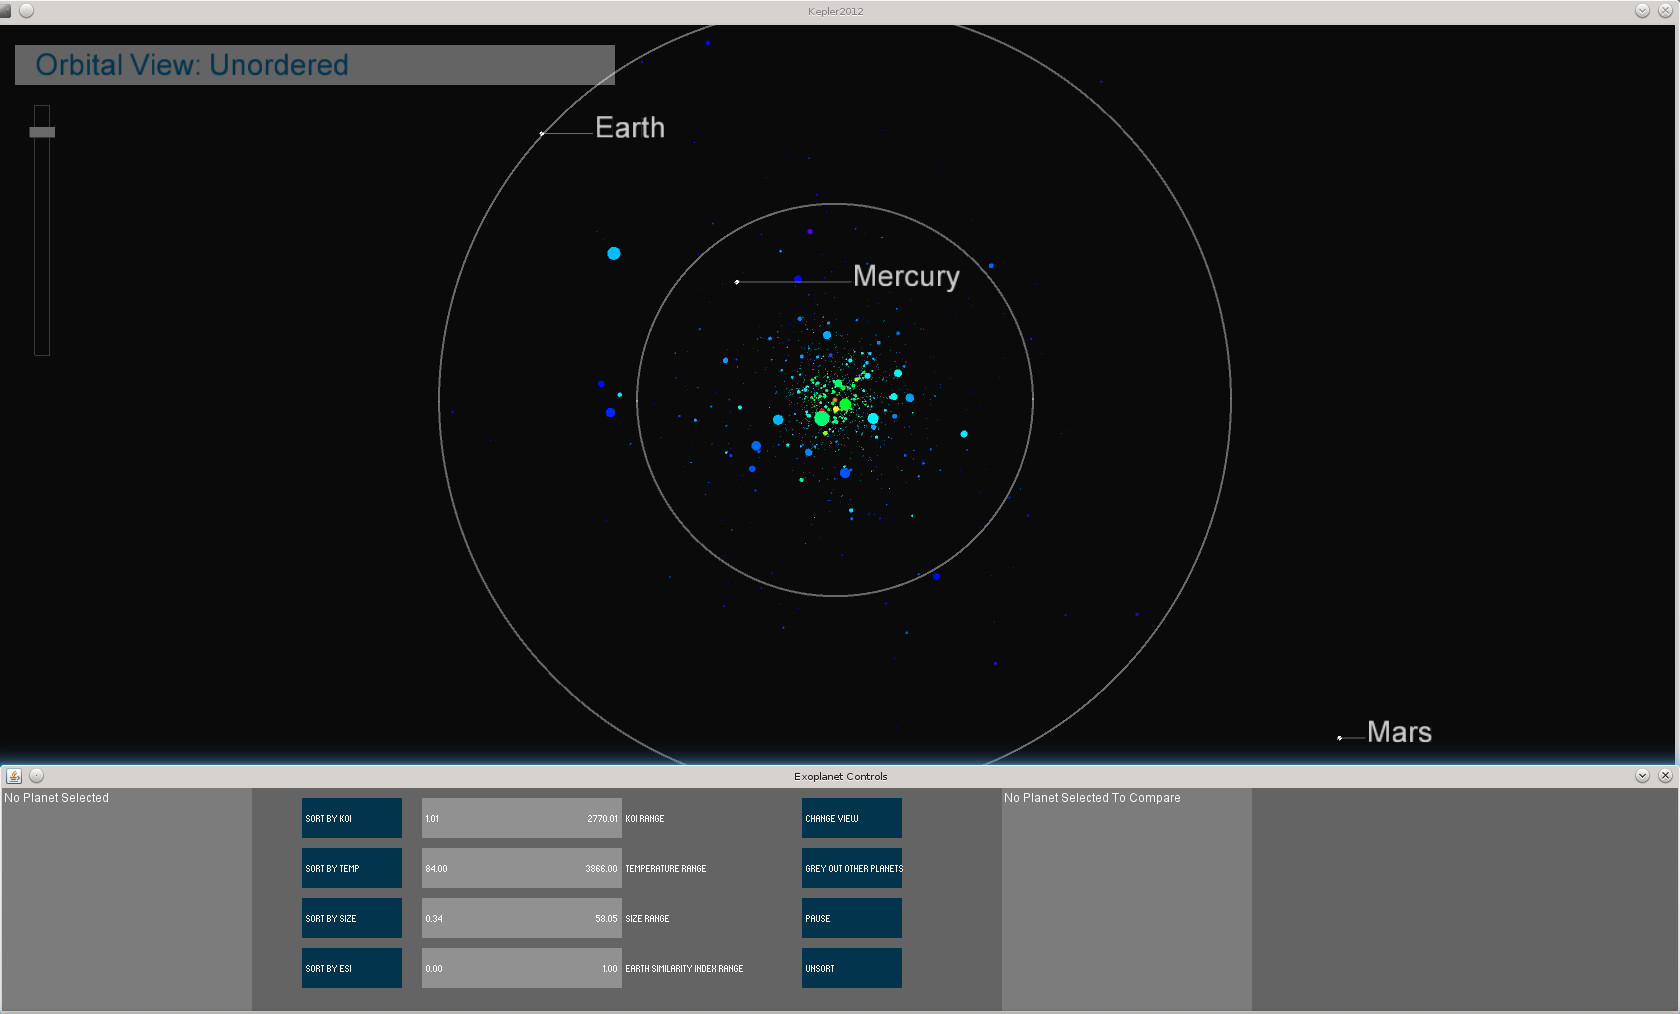
\includegraphics[width=0.8\textwidth]{images/layout_horizontal.jpg}
  \caption[Original Horizontal Layout]{Original Horizontal Layout that had an
unsuitable aspect ratio that occluded part of the visualisation.}  
    \label{fig:layoutOld}
        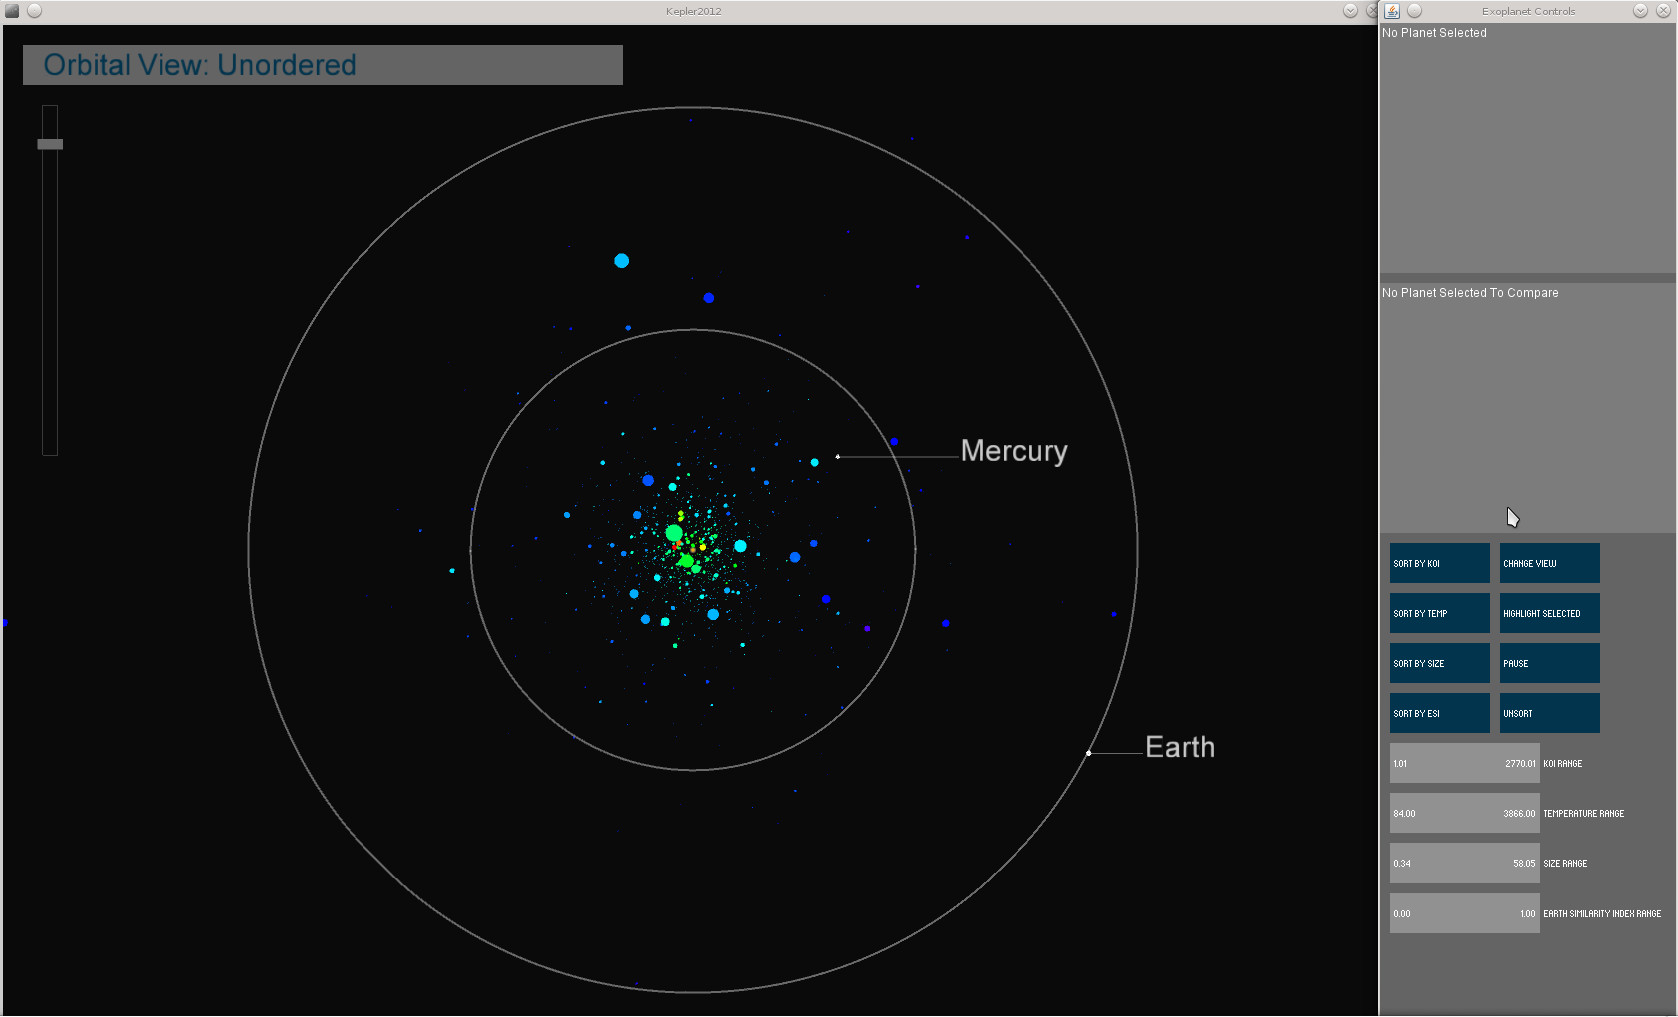
\includegraphics[width=0.8\textwidth]{images/layout_vertical.jpg}
  \caption[Improved Vertical Layout]{Improved Vertical Layout that had a higher
aspect ratio that did not hide any of the visualisation.}
  \label{fig:layoutNew}
\end{figure}

The Kinect Sensor system uses all of the features discussed above and extends it
by incorporating in gesture based control by utilising a Microsoft Kinect
sensor. Incorporate these gesture based controls was completed by specifying
gestures are detected by the visualisation which in turn modifies its state. 

\clearpage
\begin{figure}[H]
  \centering
      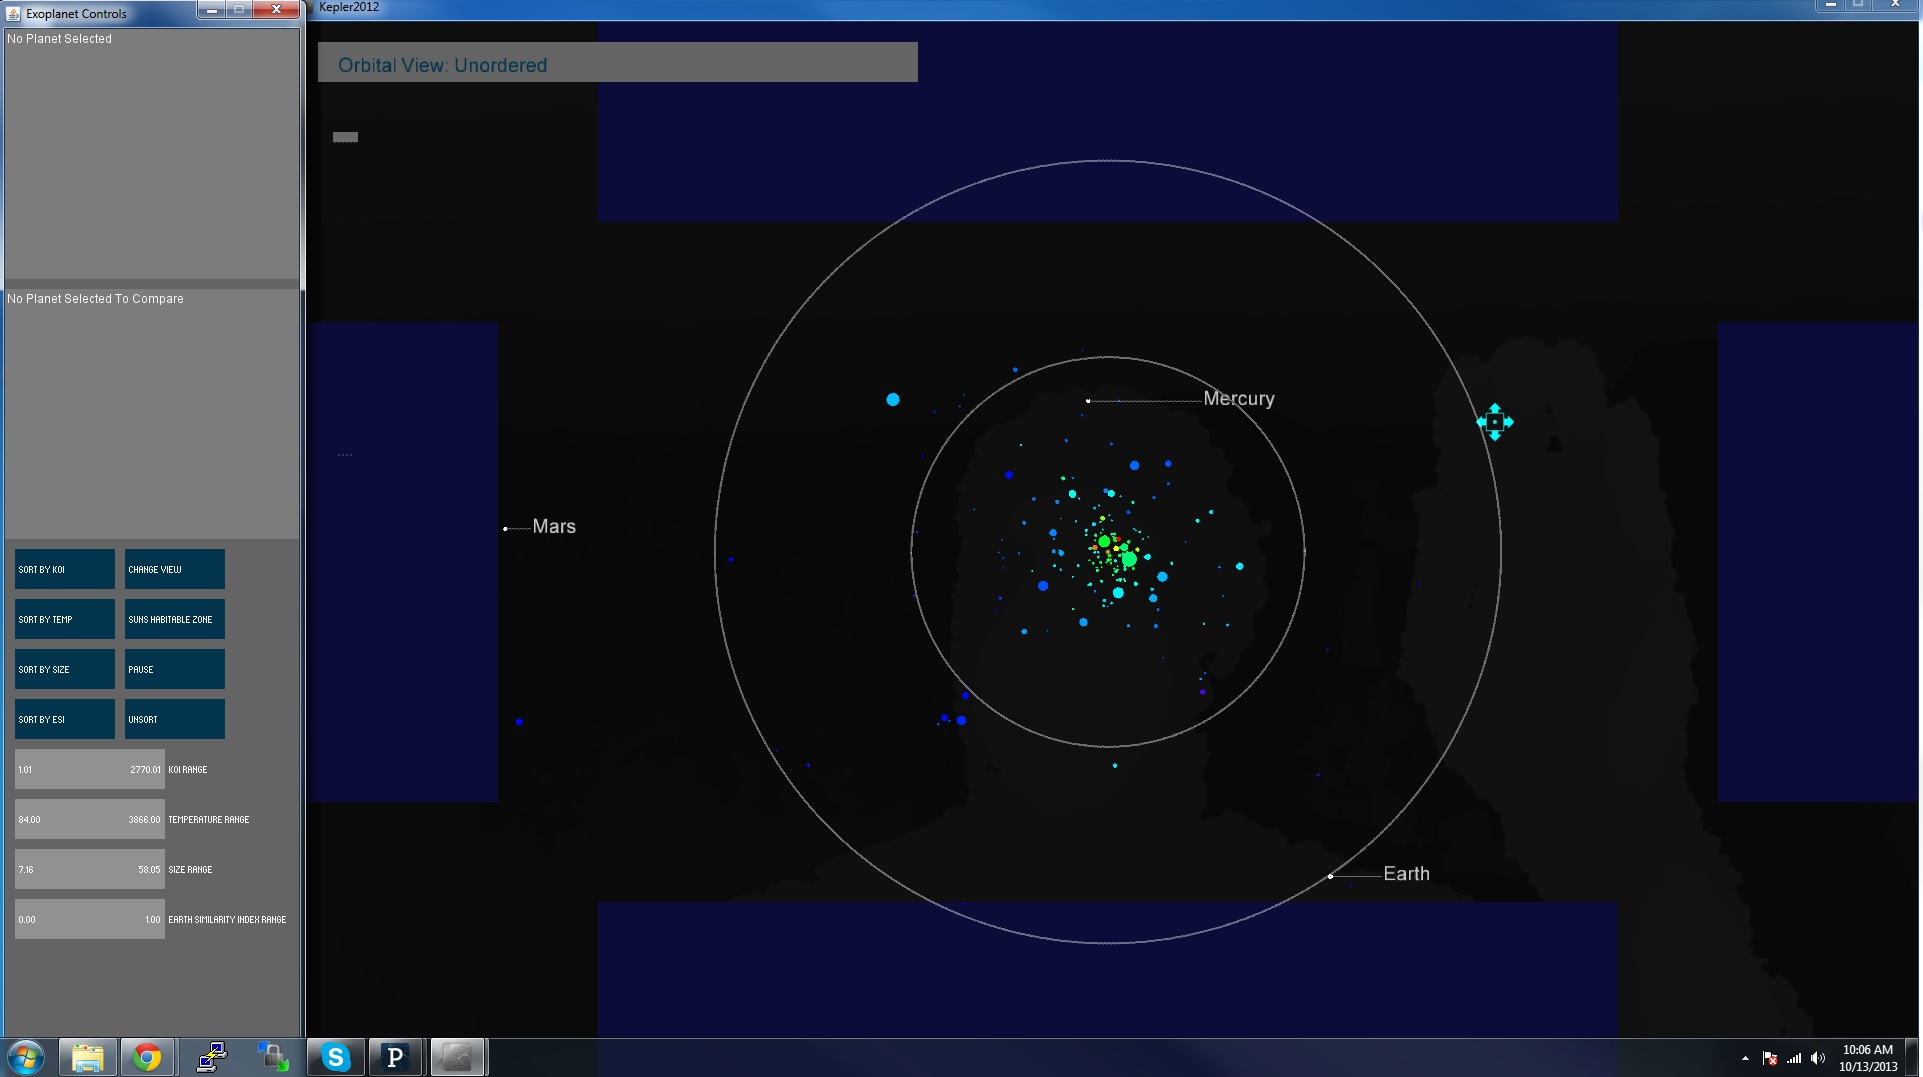
\includegraphics[width=0.8\textwidth]{images/full.jpg}
  \caption[Kinect system visualisation window]{Kinect system visualisation
window with the basic cursor visible on the outline of the users hand. Also
visible are the blue areas on the outsides of the visualisation indicating how
to perform gestures}
  \label{fig:left}
\end{figure}


As
shown in the solution design stage there were eight gestures that were needed
for the visualisation, each of which was implemented as described below

 {\bf 1. Default cursor, hand is at rest or hovering over a planet.}
\begin{figure}[H]
  \centering
      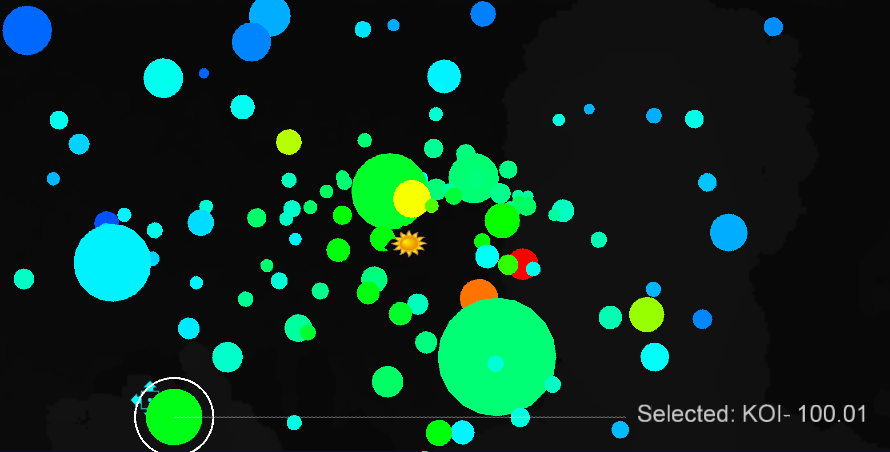
\includegraphics[width=0.8\textwidth]{images/select.PNG}
  \caption[Selecting a planet by gesture]{Selecting a planet by gesture by
hovering a hand over it. The basic cursor appears behind the selected planet.}
  \label{fig:left}
\end{figure}
\clearpage
 {\bf 2 \& 3. Panning up, hand is raised or panning down, hand is lowered.}
 \begin{figure}[H]
  \centering
      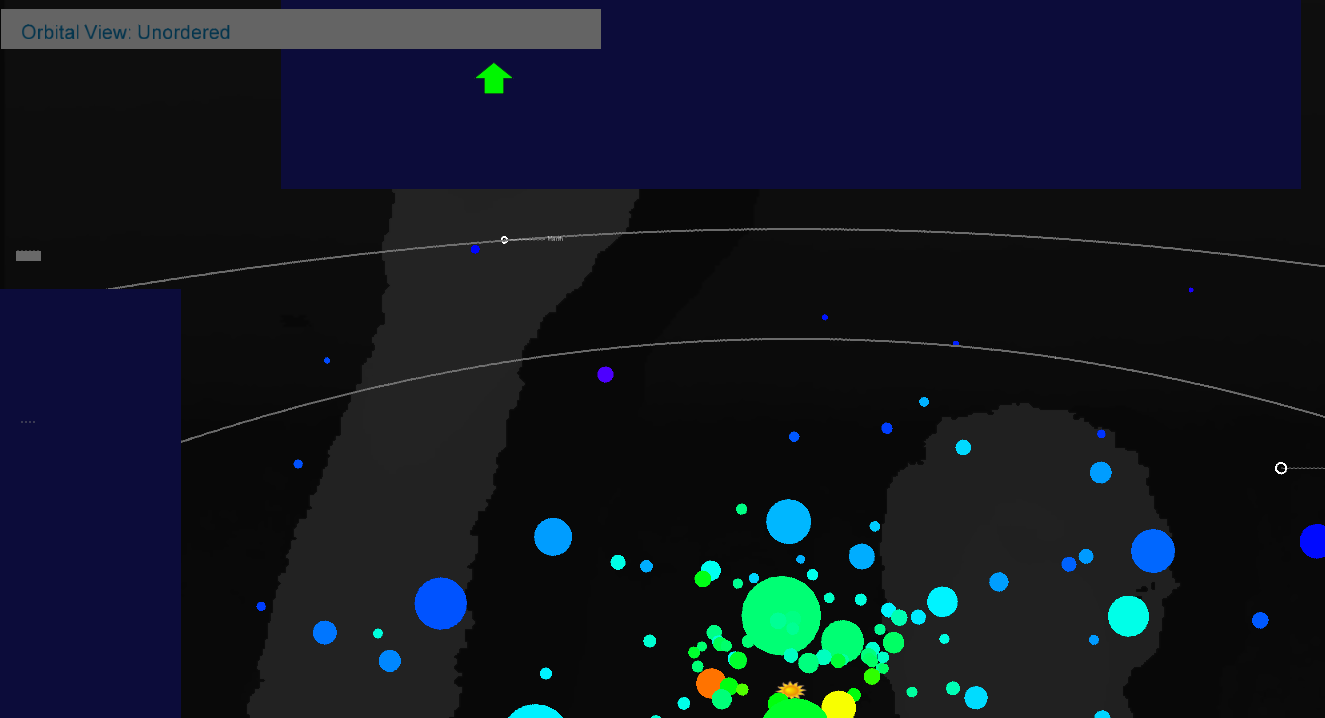
\includegraphics[width=0.8\textwidth]{images/up.PNG}
  \caption[Panning the visualisation by raising hand]{Panning the visualisation
by raising hand to the top blue area. The cursor indicates the visualisation is
panning up.}
  \label{fig:up}
\end{figure}
  {\bf 4 \& 5. Rotating left, hand is to the left or rotating right, hand is to
the right.}
\begin{figure}[H]
  \centering
      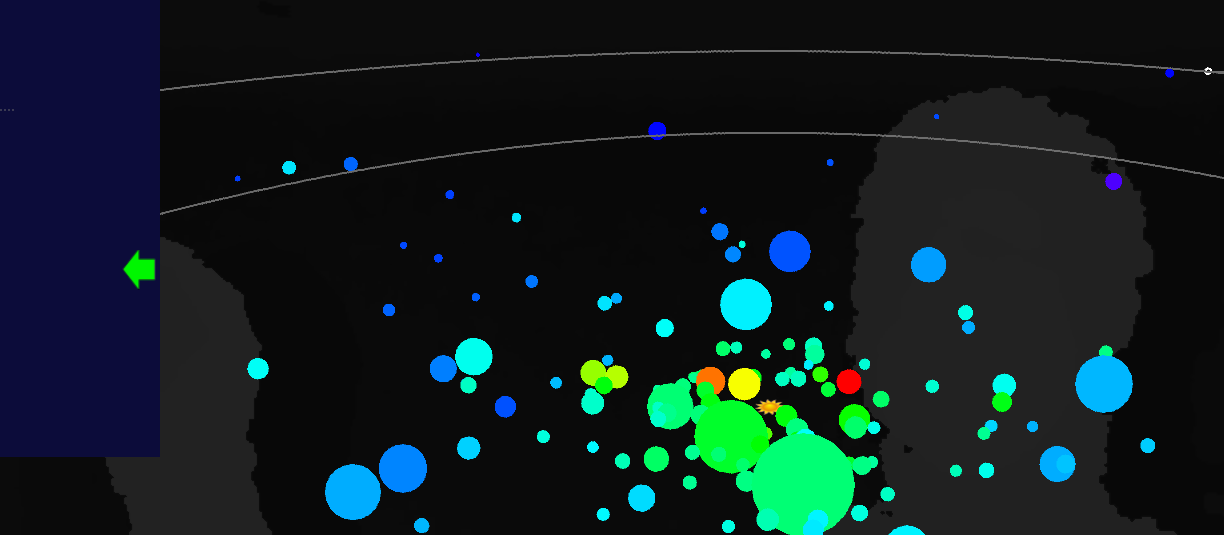
\includegraphics[width=0.8\textwidth]{images/left.PNG}
  \caption[Rotating visualisation be swiping hand]{Rotating visualisation be
swiping hand to the left of the screen. The cursor indicates the visualisation
is rotating left.}
  \label{fig:left}
\end{figure}
\clearpage
  {\bf 6. Zooming in, hand is pressed forward.}
 \begin{figure}[H]
  \centering
      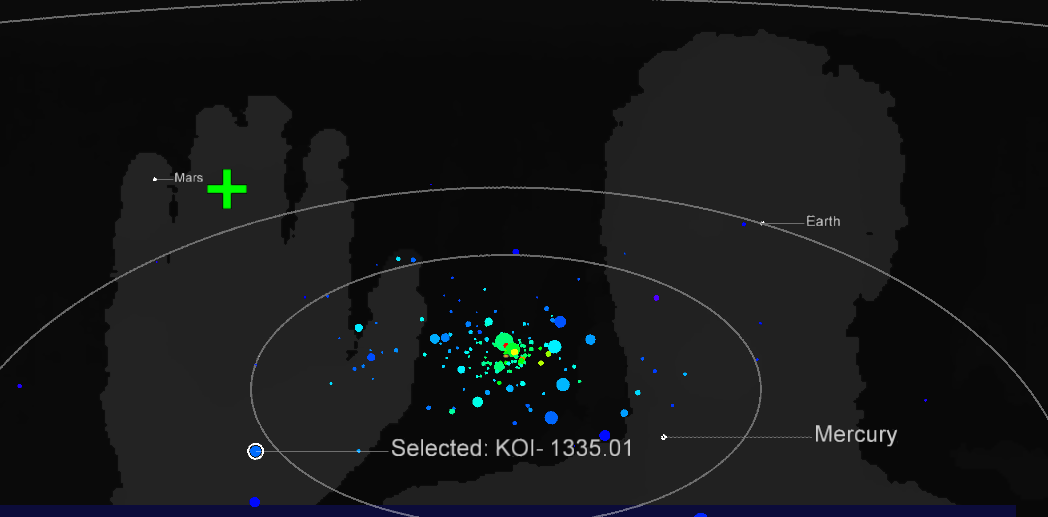
\includegraphics[width=0.8\textwidth]{images/in.PNG}
  \caption[Zooming in by pushing hand]{Zooming in by pushing hand towards the
screen. The cursor indicates the visualisation is zooming in.}
  \label{fig:in}
\end{figure}
 {\bf 7. Zooming out, hand is pulled backwards.}
\begin{figure}[H]
  \centering
      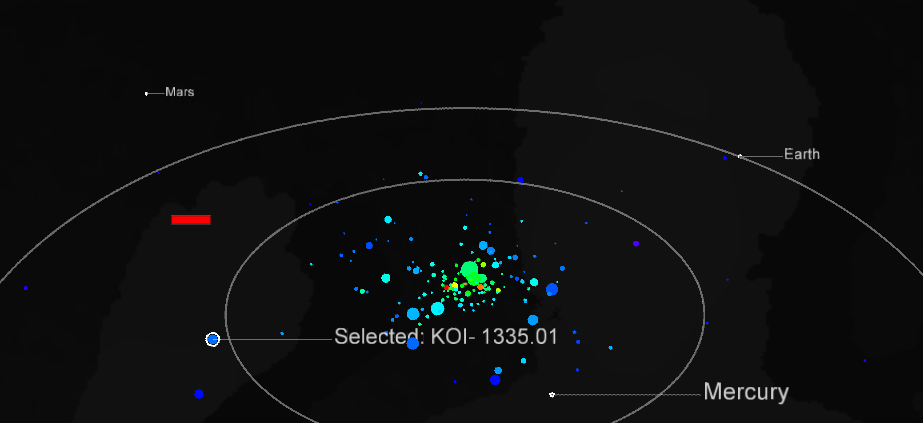
\includegraphics[width=0.8\textwidth]{images/out.PNG}
\caption[Zooming out by pulling hand]{Zooming out by pulling hand from the
screen. The cursor indicates the visualisation is zooming out.}
  \label{fig:out}
\end{figure}


In addition to this, the screen displays the user in relation to the
the visualisation, this is done by displaying a transparent outline of
the user in the background of the visualisation as can be seen in the above
figures. This is important as it gives the user a way to infer where they are
gesturing and as a way to show them that they are being detected by the system.
\\\\
Each of the features discussed were implemented using the designs created in
Chapter \ref{C:sd} to fulfill the functional requirements.
The visualisation IKVT that was created can successfully display planetary
information to convey knowledge to users (Requirement 1), allow exoplanets to be
compared against one another (Requirement 2), order exoplanets by their ESI and
by their KOI (Requirement 3), allows users to define ranges of planetary
attributes to filter which planets are displayed (Requirement 4), and view the
habitable zones of stars in
relation to the planets orbiting them (Requirement 5). These functionalities
are evaluated in the next chapter to ensure that they successfully fulfill the
functional requirements as previously stated, as well as the non functional
requirements that emphasises usability for users.




\section{Problems Encountered}

As this project builds upon a previous system, much of the existing code and
execution flow required modification. This required understanding of how the
system was originally built and designed. Because this system did not have any
unit or integration tests, going ahead without a comprehensive knowledge of the
core functionality would be have led to ineffective planning and errors being
introduced into the system. To address this, extra time and resources were
allocated to the requirements analysis and solution design stages of the
project.
\\\\
%Making use of tall of the data
Due to the number of elements that needed to be displayed on screen at any one
time (i.e. 2234 ellipses to represent the exoplanets), the load placed on the
system was very high. This uncovered a bug in
the Processing library in which the memory use of the visualisation would
periodically increase until it crashed due to an Out of Memory Exception. After
much experimentation with how to overcome this issue, I discovered that rather
than trying to render a native ellipse shape in processing, if I instead
rendered
a Scalable Vector Graphic this bug would not manifest. 
\\\\
Using the Processing framework meant using a non commercial IDE that is not
completely robust, for example when undoing multiple times in a row the file
being
modified would periodically become corrupted by lines of code being taken away
or inserted into the wrong locations. The solution to this issue was to ensure
that any changes were committed regularly to my repository on Github
\cite{github}. Doing this meant that if at any time a file became corrupted the
incorrect changes could be easily compared against the previous commit and
manually fixed. Any bugs found were reported in
the hopes that others using Processing in the future wouldn't need to address
them.
\\\\
The libraries used for gesture detection with the Kinect sensor were open-source
as this was the only way to get it to work with Processing. These open source
libraries did not have the functionality, documentation, and support that the
official Software Development Kit (SDK) that is available from Microsoft has
had. Whilst this was not a roadblock in terms of development it did mean that
more time was required for research and experimentation during implementation.
\\\\


\chapter{Visualisation Evaluation}\label{C:eval}
Following the completion of the implementation of IKVT a final
user evaluation was carried out. This evaluation was
 designed to discover whether the implemented visualisation
successfully fulfilled the requirements of the project. The evaluation
evaluation a within subjects experiment conducted with 10
participants. Each participant took turns using the IKVT with both keyboard \&
mouse and Kinect sensor whilst answering a set of questions.
The evaluation was designed to qualitatively and
quantitatively assess users
reactions and experiences with the IKVT. By mapping users experiences to the
project requirements it was possible to evaluate the success of IKVT.

\section{Purpose of Evaluation}
User studies offer a 
scientifically sound method to measure a visualisations 
performance. Studies can 
be used to evaluate the strengths and weaknesses of 
different visualisation techniques or show that a visualisation technique is 
useful in a practical sense, according to some objective 
criteria, for some specific task \cite{kosara2003thoughts}. 
The fundamental goal of conducting user studies is to 
seek insights into why particular visualisation techniques are effective
\cite{kosara2003thoughts}.


\section{Experimental Design}
\subsection{Expectations of evaluation}
An expectation in this evaluation was that users would take approximately three
minutes to feel comfortable with using the visualisation for the basic tasks of
moving the camera around, sorting the exoplanets, and using the range sliders to
filter the exoplanets. 

Following this accustomisation time it was expected that users could accurately
complete the set of questions in a worksheet (APPENDIX QUESTIONS) whilst using
the visualisation. During this stage users were expected to use both interaction
methods (Keyboard \& Mouse, and Kinect sensor). During the keyboard \& mouse
portion of the experiment the users should make more accurate selections and
exhibit more effective data seeking behavior, whereas during the Kinect portion
they would be more interested in experimenting with gestures rather than
attempting to gain information about exoplanets.

When users have finished using the visualisation and fill in the questionnaire
asking them about their experiences the expectation was that
they would detail the areas of the visualisation that they had trouble with,
felt needed improvement, and that they found useful and fun. These two forms of
results gathering provided both qualitative and quantitative results describing the
users experiences.
The expectation was that these qualitative and quantitative user results would
provide a means of viewing how successful the visualisation was in terms of
fulfilling the system requirements.

\subsection{Participants}
The user study was undertaken by 9 participants referred to as P2 to P10 as well
as 
a pilot study by a single participant referred to as P1. All were either students
or
young professionals from a mix of specialties, aged between 21 and 26 with a
mix
of genders of 5 females and 4 males. 5 of these participants had extensive
prior experience with Kinect sensors, and all participants had experienced a 3D
visualisation before. Only 6 out of 10 participants had knowledge of the
exoplanets discovered by the Kepler telescope.

\subsection{Evaluation Environment}
\begin{figure}[H]
  \centering
      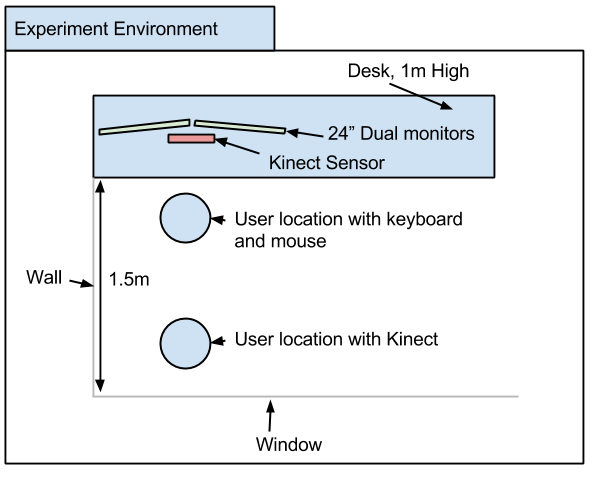
\includegraphics[width=0.8\textwidth]{images/environment.png}
  \caption{Evaluation environment}  
    \label{fig:environment}
\end{figure}


\subsection{Evaluation Method}
A poorly designed experiment will only yield results of limited value, because
of this it was important to ensure that each stage of the experiment was
focused on evaluating a specific area of the visualisation in relation to the
project requirements. There were 3 key methods of gathering results during this
evaluation; a
worksheet to fill out whilst using the visualisation made up of 2 sets of
questions(one for the keyboard \& mouse system and one for the Kinect
system)(APPENDIX), a questionnaire to
fill in afterwards about the experience (APPENDIX), and the examiners
observations about
how the users interacted with the system.  
\\\\
The following are the steps that were carried out during each user evaluation to
ensure that the variables were the same each time
\begin{itemize}
\item The participant enters the room and sits down at the computer.
\item They are handed the consent form and information sheet.
\item After these are completed they are handed the user questionnaire and the
set of questions to answer while using the system. On this questionnaire there
are two sets of questions, the first is for the keyboard \& mouse system, and
the second if for the Microsoft Kinect system.
\item They are then given a brief introduction into each of the visualisation
components and what the visualisation as a whole represents
\item Following this they are advised that they have 5 minutes to get
familiarised with the system but they do not need to use all of this time (the
amount of time taken will be recorded for analysis of how user friendly and
intuitive the system is).
\item Following this the participant is asked to complete the worksheet by first
using the mouse and keyboard system. When they feel they have answered the first
set of questions they will notify the examiner who will move the user to the
Kinect
system to continue with the second set.
\item Once the participant has completed both sets of questions they are asked
to fill
in the qualitative user questionnaire about their experiences using the
visualisation. 
\item Following this if the examiner has no follow up questions the user is free
to leave.
\end{itemize}

\subsection{Pilot Study}
Due to the significant costs associated with running an experiment, it 
is valuable to conduct a pilot study with one or two 
participants. This allows testing and refining of the experimental
design before starting a full-fledged study with numerous 
participants \cite{kosara2003thoughts}. 

The reason for conducting a pilot study for this project was to ensure that
the experiment was producing the data needed to evaluate IKVT as well
as taking the correct amount of time to complete. It was also
used to discover whether any aspects of the study would
interfere with the results. One participant was asked to take part in a pilot
study, this participant is referred to as P1. P1 was asked to complete all of
the activities that
make up the main experiment. This pilot study took approximately 15 minutes as
intended including the time needed for the explanation and completion of
paperwork, as well as the experiment itself.

P1 successfully completed each of the questions in the worksheet whilst using
the visualisation with only
limited assistance from the examiner. This assistance was required due to the
wording of
some of the tasks being ambiguous which caused
unnecessary confusion which could have interfered with the results. These
ambiguous questions and
tasks were removed prior to the main user study. During the main study only P4
and P10 asked for clarification on the questions or tasks.

P1 had some initial difficulty using the range sliders but after a small period
of experimentation began using them for the majority of tasks which turned out
to be effective. P1 also found that whist the range sliders were useful,
they did not allow fine enough control for making small changes to the filters.
The component
of the visualisation that P1 had the most difficulty with was using the
Goldilocks
view. This difficulty seemed to stem from the lack of a common point of
reference for each planet due to each planet having a different star with its
own Goldilocks zone.

During the Kinect portion of the experiment P1 found that being in a sitting
position whist interacting with the visualisation did not feel natural due to
``being required to reach out and exert effort to hold an upright position of
the arms for an extended period of time''. The following figure displays P1s
quantitative results from the questionnaire.
\begin{figure}[H]
  \centering
      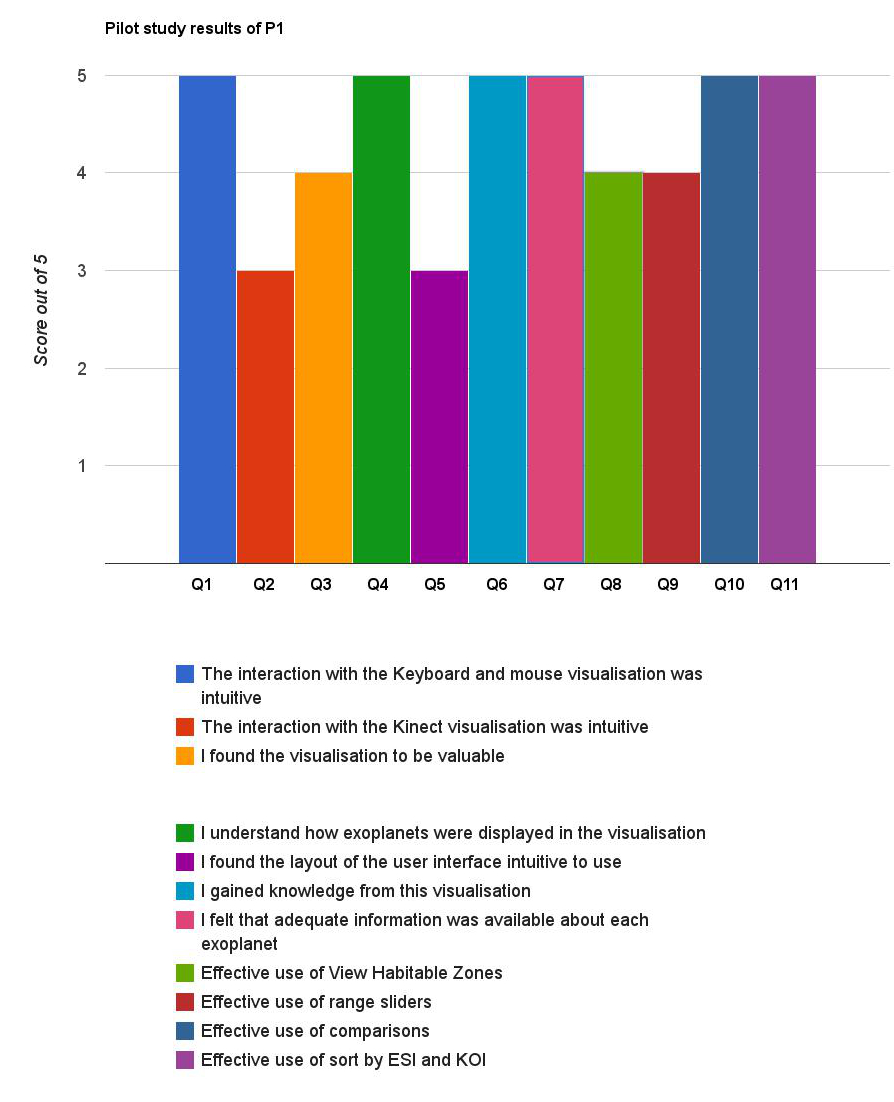
\includegraphics[width=1\textwidth]{images/pilot.jpg}
  \caption{Pilot study results of P1}  
    \label{fig:pilot}
\end{figure}

\section{Results}
The keyboard \& mouse portion of the experiment was primarily intended to
evaluate how the interaction techniques introduced into the
visualisation aided users in their information seeking behavior.
This was evaluated through the first part of the worksheet filled
in by users whilst using the visualisation. These questions were designed in a
way that
encouraged users to make use of each of the interactive features that was
implemented as part of this project.

The Microsoft Kinect portion of the experiment was intended to evaluate how
users would react to interacting with the visualisation by gesture. The
worksheet for this portion of the evaluation were designed to find out whether
users could successfully navigate the visualisation without keyboard \& mouse.
The following subsections discuss the qualitative and quantitative results of
this evaluation. 

\subsection{Qualitative Results}
\subsubsection{Evaluation of Functional Requirements}
\begin{enumerate}
{\bf
 \item[R1.] The visualisation needs to display planetary information to convey
knowledge to users.}

The experiment demonstrated that the increased amount of information available in IKVT
 about each exoplanet allowed participants to access
more information contained in the Kepler Exoplanet database than in the existing
system. All participants were able to successfully complete the worksheet
questions
that involved accessing information about exoplanets stored in the
text areas in the interaction panel.
P8 found that a weakness of the system was the amount of concepts that needed
to be understood about exoplanets and so including a glossary would be an
improvement. A glossary would allow users to discover the meaning to any terms in the visualisation mitigating the risk of user
confusion.

All participants reported learning something from the visualisation that they
did not previously know, and those who had no knowledge of exoplanets prior to
the experiment felt that they had learned something valuable. For example P4
felt that using IKVT broadened her perception of how much information we know
about planets so far away.


{\bf
 \item[R2.] The visualisation needs to allow exoplanets to be compared against
one another.}

Whilst all participants used the comparison functionality during the
familiarisation stage, only 3 of the participants used it while completing the
worksheet. This could be because it was not made obvious enough, or because the
questions asked of users did not force users to use this feature to get an
answer. When the participants did use the comparison tool they were able to use
it successfully and most tried it multiple times with multiple exoplanets. P3
found that being able to compare the exoplanets against one another was useful
as he could leave an interesting exoplanet selected whilst comparing it against
multiple other exoplanets. He found that it was easy to compare the information
for each exoplanet and to get a sense of the attributes of exoplanets.

{\bf
 \item[R3.] The planets need to be able to be ordered by their similarity to
earth (ESI) and by their Kepler Object of Interest number (KOI).}
 
All participants used the sort by KOI and ESI functionality effectively without
any confusion. P8 liked being able to toggle between the different attributes
sortings as he found that it gave a clearer view of the attributes in a visual
manner rather than needing to look at the text areas.
P7 found the exoplanets sorted by ESI to be the most interesting view. She
spent an extended period of time experimenting with this during question 8 of the
worksheet before moving on the later questions. P7 stated that she could find
the potentially habitable planets easily as she could assume that they would
need to be similar to Earth which the visualisation clearly showed.

{\bf \item[R4.] The visualisation needs to allow users to define ranges of
planetary attributes to filter which planets are displayed.}

All participants successfully used the range sliders whilst completing the
worksheet questions. The range sliders were used frequently by all participants to discover the
exoplanets that were the outliers in regard to their attributes (ie, high
temperatures). 3 out of 10 participants had trouble when moving between
questions on the worksheet due to forgetting
to reset the range sliders after using them and thus only a subset of the
exoplanets were displayed. 
P5 found the zooming effect that occurred when planets were filtered useful for making more accurate selections and spent time
experimenting with it. P6 found that being able to sort the planets according to
attributes and
then filtering them to remove the planets she did not want was a powerful tool.

{\bf \item[R5.] Users need to be able to view the habitable zones (Goldilocks zones) of stars in
relation to the planets orbiting them.}

The evaluation of this requirement showed that whilst the functionality was
successfully implemented it lacked usability. All but one user in the study
found that this was because it was unintuitive. What caused this was that the
Goldilocks zone of each star is different. This meant that each time a user
selected a new exoplanet the location of each of the zones changed as was
intended. However, this confused all but one user as they were expecting the
zones to stay the in the same locations.  

\end{enumerate}

\subsubsection{Evaluation of Nonfunctional Requirements}
\begin{enumerate}
 {\bf\item[R6.] All interaction methods must be visible and intuitive.}
 
The experiment found that all interactive methods were able to be seen and used
by users. However due to the design of the components being low key as to not
draw attention away from the main visualisation, the participants often forgot
about them, especially as the interaction panel was at the side of the screen.
For example P5 found that because the information panel was not central in the
visualisation
it required effort to break away from the main visualisation window and thus broke
the immersion. Another issue found was that the text of the components in the
interaction was to small for some users to see clearly and quickly.
A common consensus was that the layout of the interactive components were fine
but could be improved by making them ``pop out more'' especially as many
participants didn't initially spot the text areas changing as planets were selected
until reading the worksheet questions.
 
{\bf \item[R7.] The visualisation must remain uncluttered to reduce information
overload.}

All users felt that the amount of information displayed in the
visualisation was appropriate apart from P7 who felt
it displayed to much information at once which caused confusion. P10 felt that
the interaction panel contained the right amount of information, but felt that
it could be improved by changing its design to make it stand out more and
emphasis each component contained in it. P4 felt that the names of some of the
attributes were not made clear enough (E.g. ESI, KOI). P5 felt that limiting the
amount that the camera could move would be an improvement,
especially in the graph view where their is a fixed plane where content is displayed..

{\bf \item[R8.]  There needs to be two modes of interaction in the system,
keyboard \& mouse vs gesture based.}

The experiment found that both the interactive mediums had different
strengths and weaknesses. The keyboard \& mouse system was the most effective
for information seeking as it provided more accuracy and was easier to use the
interaction panel elements. The Microsoft Kinect system was worse for discovering
information, but it was the most fun out of the two options due to its novelty.
All of the users felt that had they had more time with the Kinect system, they
would have been more effective at accessing the information available. This was
because they were preoccupied performing basic actions like moving the camera
and selecting planets due to the short time available. For example P6 found that
she used more time playing around with the Kinect system trying to select
planets rather than trying to get information. All participants but P4 felt that
the visualisation responded with the appropriate actions and magnitudes for each
gesture. P4 expected the magnitude of the visualisation changes to be more
than they were, ie it should have rotated faster. P6 felt that there needed to
be more physical movement space in which to use the Kinect as some movements felt
cramped. Another weakness discovered about the Kinect sensor was that it
detected the whole hand rather than a more controllable area like a finger.
P10 found that overlapping planets made it hard to make selections with the
Kinect and that he needed a way to cancel a selection without having to select
another planet.

\end{enumerate}

\subsection{Quantitative Results}
\subsubsection{Evaluation of Functional Requirements}

A key part of this visualisation is that it should be intuitive enough that a
user can walk up to it and feel comfortable using it to explore data within a
short period of time. The results showed that some users felt that they could
effectively use the visualisation very quickly (within 1 to 4 minutes) whilst
others took longer (up to 5 minutes) as Figure \ref{fig:comfort}. 
\begin{figure}[H]
  \centering
      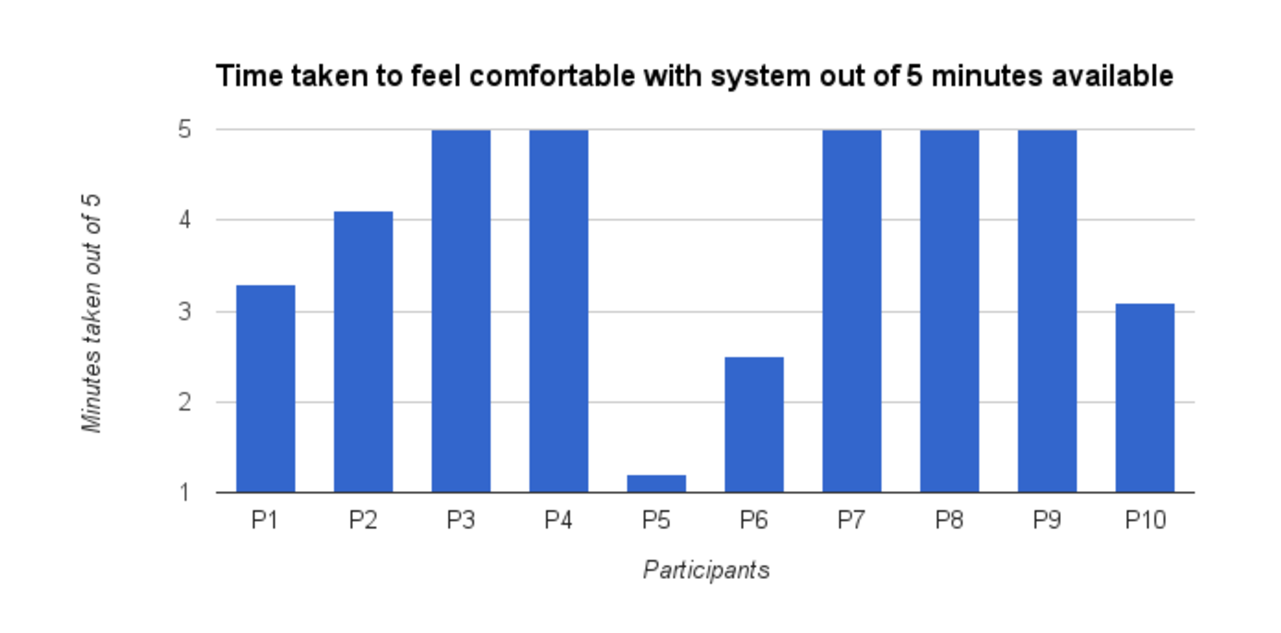
\includegraphics[width=1\textwidth]{images/comfort.pdf}
  \caption{Amount of time taken out of a possible 5 minutes for users to feel
comfortable with
visualisation before moving onto the worksheet. }  
\label{fig:comfort}
\end{figure}

As we can see below in Figure \ref{fig:summary} all users performed well in all
aspects apart from with ``Req: 5 Effectively used habitable zones'' which the
qualitative analysis also found. Another notable result was that the keyboard \&
mouse was rated as more intuitive than the Kinect sensor, again this is
supported by the qualitative results. Apart from these key areas of interest the
results are as expected with each area being scored highly. 
\begin{figure}[H]
\centering
      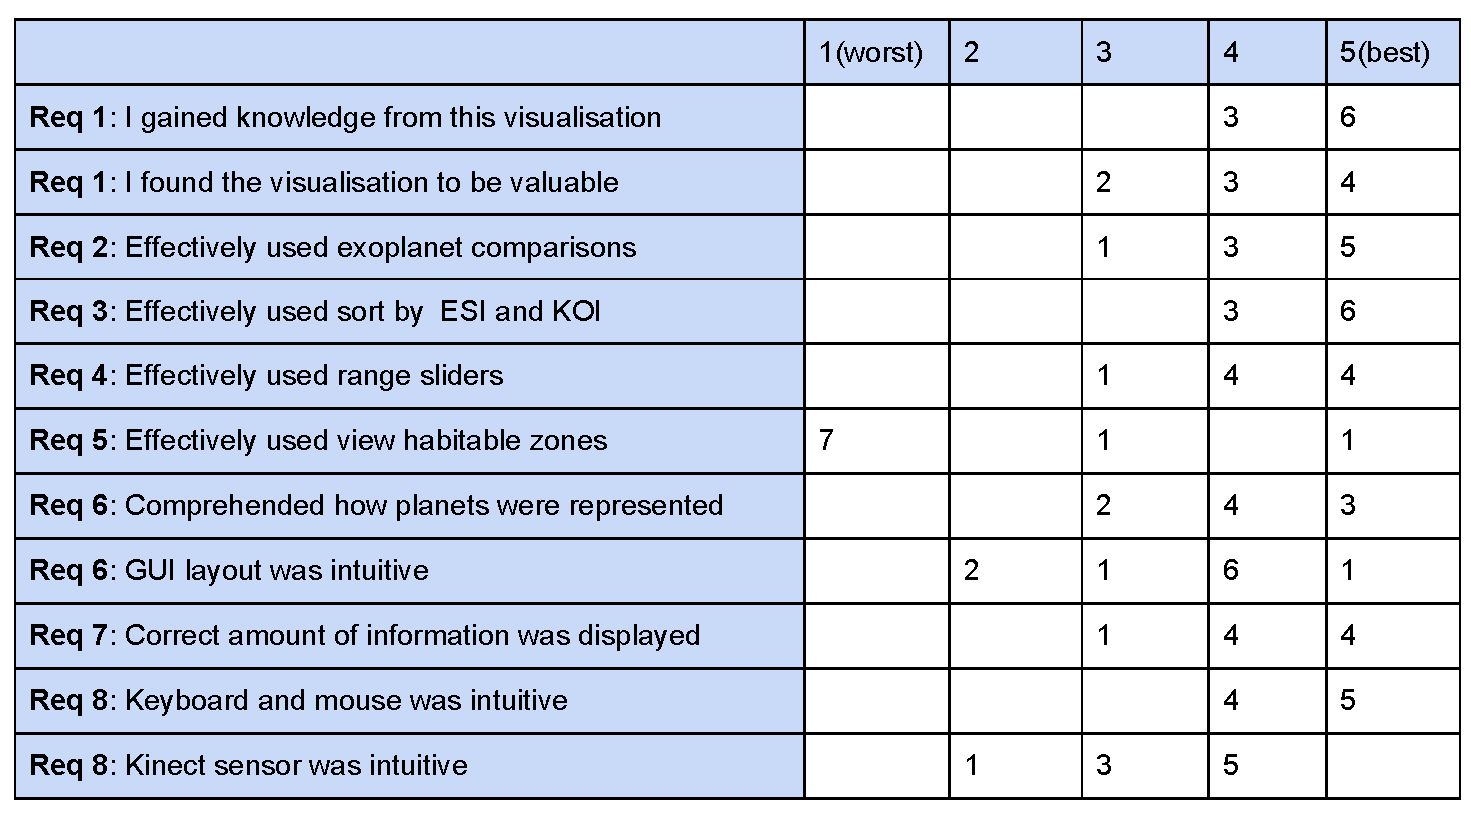
\includegraphics[width=1\textwidth]{images/summaryResults.pdf}
  \caption{Summary of the quantitative results gathered from participants.}  
    \label{fig:summary}
    \end{figure}
    
Seeing how different participants scores attribute to the table in Figure
\ref{fig:summary} helps to understand the distribution of scores. As Figure
\ref{fig:breakdown} shows, some users consistently gave higher or lower scores
which could have caused a bias in the results. However it does show that some
users enjoyed using the visualisation whilst others did not. 
    
\begin{figure}[H]
  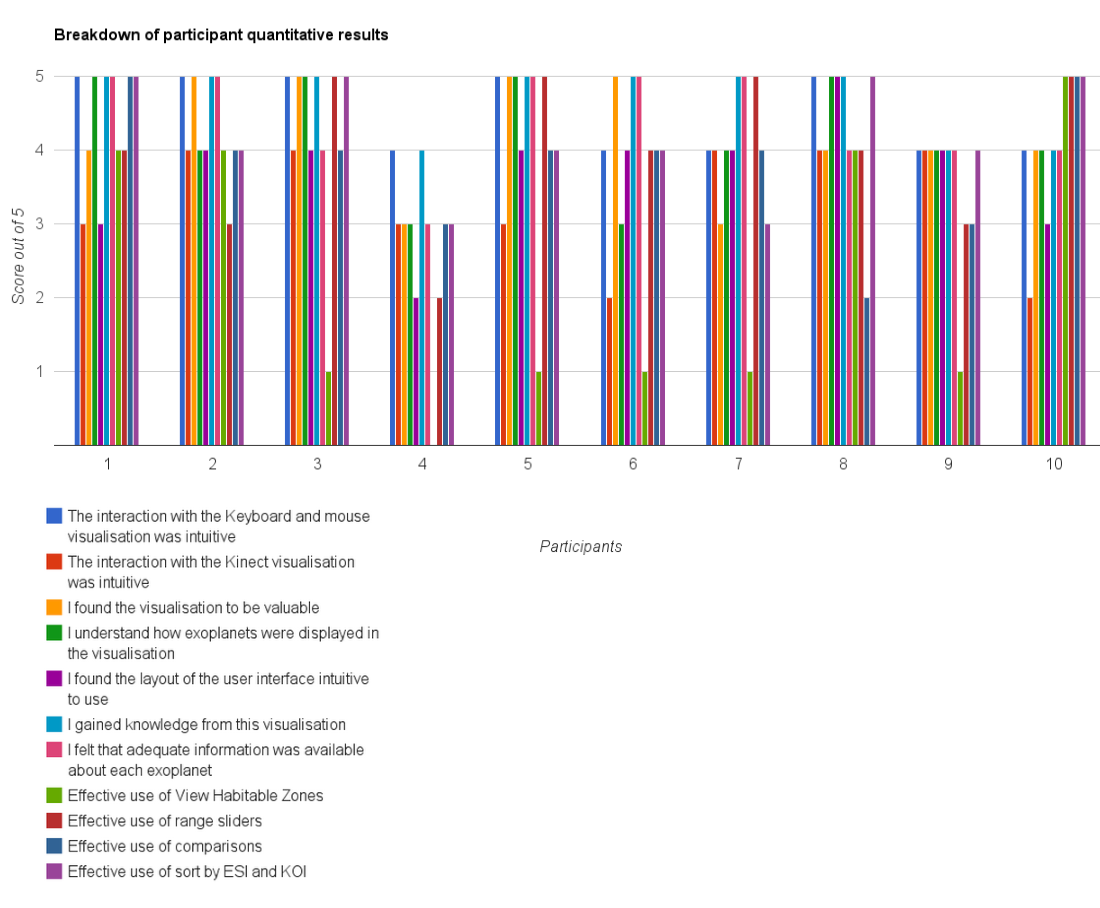
\includegraphics[width=1\textwidth]{images/breakdown.pdf}
  \caption{Breakdown of quantitative results between users}  
    \label{fig:breakdown}
\end{figure}

\section{Discussion}
\subsection{Threats to Validity}
A key factor in this user evaluation was the small number of users
chosen due to the time limit of 300 hours which did not allow for a larger more
in depth study. Because of this, the results gathered may
not be representative of a larger population. It was also limited to a narrow
demographic of young professionals and students which does not cover all of the
intended users of IKVT. To amend this, the population of this study would need to
be expanded to contain age ranges above and below those in this study.

A further threat to the validity of this evaluation was the limit placed on
participants for the familiarisation stage. Some participants may have required
even more time than the 5 minutes alloted for. By cutting the familiarisation
stage off at this point it may have caused some participants to be unprepared
to carry out the completion of the worksheet and thus skewing the results.

\subsection{Potential Improvements}
Due to the negative results surrounding the viewing of Goldilocks zones,
this area of the evaluation should be analysed further to determine whether the
tasks in the evaluation relating to it were flawed, or whether the functionality
and its design were flawed. To discover this it would be important to evaluate
the questions used in the study to determine whether or not they skewed the result or if the the functionality needs to be
redesigned. 


\section{Summary of Evaluation}
This evaluation of IKVT provided several key results and insights into the
success of IKVT. The general consensus by the participants of the study
was that the system had a low learning curve, was enjoyable to use, and allowed
access to interesting information. Participants also agreed that the Kinect system was more fun to use than the keyboard \&
mouse because of its novelty, but lacked the control that the
keyboard \& mouse allowed which made it less effective at accessing the
information in the visualisation. The keyboard \& mouse was found to the be the
most effective method for navigating the visualisation because of the amount of
control that it offered users as well as being the interactive medium that
participants had the most experience with.

The evaluation revealed one problem area in the visualisation that was related
to Requirement 5 (Users need to be able to view the habitable zones of stars in
relation to the planets orbiting them), and Requirement 6 (All interaction
methods must be visible and intuitive). This problem occurred because users found that
viewing where each exoplanet was located in relation to their stars habitable
zones was unintuitive and difficult to use. This result could have occurred for a
range of reasons, the most likely being that the evaluation questions were
counterproductive to using this functionality, or that the functionality itself
is flawed.

This user study served to evaluate how effectively IKVT could convey the
information in the Kepler Exoplanet dataset. The findings pointed to it
being successful in this regard. However, there are areas that this evaluation
could be improved to strengthen this result. The main improvement for this
evaluation is to include a larger number of participants more representative of
the wider population.




\chapter{Summary}\label{C:con}
This project contributes the design,
implementation, and evaluation of an
interactive 3D visualisation called the Improved Kepler Visualisation Tool
(IKVT) to the field of Human Computer Interaction. IKVT has two modes of
interaction; the traditional keyboard \& mouse and
the more novel Microsoft Kinect sensor. 

\section{System Design}
The requirements for IKVT were designed using Cooper et al.'s user oriented
design approach which emphasised using user models and user scenarios
\cite{AboutFace3}.  Two user
models and seven user scenarios were used in the creation of eight project
requirements that
were used extensively in the design, implementation and evaluation of IKVT to
ensure that it
solved the four key issues that this project hoped to address.
\begin{description}
 \item[Issue 1.] Content in the Kepler Exoplanet Database is difficult to view
and
understand due to its amount and labeling.
 \item[Issue 2.] Planetary information is complex and difficult to comprehend
without
a visual reference due to its scale.
 \item[Issue 3.] Existing visualisations for exploring planetary data have
minimal
functionality for exploring the information in effective ways.
 \item[Issue 4.] Visualisations need to allow user interaction to make the most
of the data they display.
\end{description}


The solution designs created were used to guide the implementation of IKVT to
ensure that it completed each of the system requirements. Using class and
sequence diagrams provided a means of understanding the existing system in terms
of its structure and execution. The designs were used to guide the aesthetics of
each of the functionalities produced. 
\section{System Implementation}
IKVT was implemented in Processing, an open-source Java programming language and
integrated development environment (IDE). It was built upon an existing
visualisation, the Kepler Visualisation Tool \cite{kepler_github,
kepler_article} to create more effective interaction techniques and allow users
to access more information in the Kepler Exoplanet dataset. During the
implementation stage of the project each of the
designs created in the system design stage were implemented in
fulfillment of the project requirements. 

\section{System Evaluation}
IKVT was evaluated in a user study that gathered both qualitative and
quantitative
results. The evaluation was designed to gather users experiences with the IKVT
to examine whether or not it fulfilled the system requirements designed to solve
the issues mentioned above.

The evaluation found that all of these requirements were fulfilled by the
visualisation. In addition to this the participants in general found that the
IKVT had a low learning curve, was enjoyable to use, and allowed
access to interesting information. There was also a common consensus among the
participants that the Kinect system was more fun to use than the keyboard \&
mouse because of its novelty, but lacked the control that the
keyboard \& mouse allowed which made it less effective at accessing the
information in the visualisation. The evaluation also revealed that one area,
viewing the habitable zones of stars, lacked
usability because it was unintuitive for the users participating in the
evaluation.     
\section{Future Work}
IKVT  can be taken further in many ways depending
on how it is intended to be used. There is the option of using the system as a
terminal that users would use at an observatory or attraction where prior
knowledge of the system is limited and amount of time users would spend on the
system would be small. In this case further expanding the user experience and
improved Kinect interaction would be beneficial as immersion would be the
decider on its success. Another option would be for a standalone
desktop system that users would use multiple times and so prior knowledge of how
to use the system could be expected. This would mean that more complex
functionality could be introduced with the expectation that it could be learned
and used by
users. The systems current state could me modified to fit into either of these
two options.

A weakness in the system that needs to be addressed is the Goldilocks zone view
which the evaluation discovered was not intuitive enough to make it effective.
To
address this the functionality needs to be evaluated to discover which aspects
of it cause it to be unintuitive. The first improvement is to provide a common
point of reference for the habitable zones. This is because the area that
confused users the most was that when they selected a new planet Goldilocks
zones changed. 

The user evaluation found that gesture based control of IKVT was the most
enjoyable way for users to interact with IKVT even though it was less effective
at accessing information. This opens up the opportunity for further work to
improve the level of gesture based control and accuracy so that it rivals the
keyboard \& mouse. This could be done in a range of ways from simply enhancing
the intuitivity, to more advanced methods of gesture detection such as joining
gestures together.
\\\\ 
These three future improvements are ordered by importance below.
\begin{enumerate}
 \item Address Goldilocks zone view
 \item Improve gesture based control
 \item Focus IKVT towards a set environment to focus further development
\end{enumerate}

\section{Project Contributions}
This project delivered an interactive 3D visualisation that conveys more
information and contains interactivity to allow users to access more of the
information contained in the Kepler Exoplanet dataset than other visualisations
in the same field. This
extension was evaluated both qualitatively and quantitatively by a within
subjects user experiment with the results indicating that it fulfilled the
requirements.
A key part of this project was the development of interactive techniques to
provide improved access to this data. These techniques are a mix of keyboard and
mouse as well as a novel gesture based approach using a Microsoft Kinect sensor.
The work and research completed for this project will provide the opportunity
for further improvement of the produced visualisation in the future.



%%%%%%%%%%%%%%%%%%%%%%%%%%%%%%%%%%%%%%%%%%%%%%%%%%%%%%%

\backmatter

%%%%%%%%%%%%%%%%%%%%%%%%%%%%%%%%%%%%%%%%%%%%%%%%%%%%%%%
 

%\bibliographystyle{ieeetr}
% \nocite{*}
\bibliographystyle{acm}
\bibliography{refs}
\appendix
\clearpage
\chapter{Project Gantt Chart}
\label{ap:gantt}
\begin{figure}[H]
  \centering
      \includegraphics[width=1.3\textwidth,angle=90]{images/gantt.jpg}
  \caption{Gantt Chart used for project}
\end{figure}

\chapter{Ethical Approval for User evaluation}
\section{Information Sheet for Experiment}
\label{ap:info}
\includepdf[pages={-}]{evaluation/OwensHonorsInformationSheet.pdf}

\chapter{Consent Form for Experiment}
\label{ap:consent}
\includepdf[pages={-}]{evaluation/OwensHonorsConsentForm.pdf}

\chapter{Worksheet for Experiment}
\label{ap:work}
\includepdf[pages={-}]{evaluation/worksheet.pdf}

\chapter{Questionnaire for Experiment}
\label{ap:quest}
\includepdf[pages={-}]{evaluation/OwensHonorsUserQuestionaire.pdf}

\chapter{Ethical Approval for Experiment}
\label{ap:approval}
\includepdf[pages={-}]{evaluation/ethicsAproval.pdf}


\end{document}
